\documentclass[1p]{elsarticle_modified}
%\bibliographystyle{elsarticle-num}

%\usepackage[colorlinks]{hyperref}
%\usepackage{abbrmath_seonhwa} %\Abb, \Ascr, \Acal ,\Abf, \Afrak
\usepackage{amsfonts}
\usepackage{amssymb}
\usepackage{amsmath}
\usepackage{amsthm}
\usepackage{scalefnt}
\usepackage{amsbsy}
\usepackage{kotex}
\usepackage{caption}
\usepackage{subfig}
\usepackage{color}
\usepackage{graphicx}
\usepackage{xcolor} %% white, black, red, green, blue, cyan, magenta, yellow
\usepackage{float}
\usepackage{setspace}
\usepackage{hyperref}

\usepackage{tikz}
\usetikzlibrary{arrows}

\usepackage{multirow}
\usepackage{array} % fixed length table
\usepackage{hhline}

%%%%%%%%%%%%%%%%%%%%%
\makeatletter
\renewcommand*\env@matrix[1][\arraystretch]{%
	\edef\arraystretch{#1}%
	\hskip -\arraycolsep
	\let\@ifnextchar\new@ifnextchar
	\array{*\c@MaxMatrixCols c}}
\makeatother %https://tex.stackexchange.com/questions/14071/how-can-i-increase-the-line-spacing-in-a-matrix
%%%%%%%%%%%%%%%

\usepackage[normalem]{ulem}

\newcommand{\msout}[1]{\ifmmode\text{\sout{\ensuremath{#1}}}\else\sout{#1}\fi}
%SOURCE: \msout is \stkout macro in https://tex.stackexchange.com/questions/20609/strikeout-in-math-mode

\newcommand{\cancel}[1]{
	\ifmmode
	{\color{red}\msout{#1}}
	\else
	{\color{red}\sout{#1}}
	\fi
}

\newcommand{\add}[1]{
	{\color{blue}\uwave{#1}}
}

\newcommand{\replace}[2]{
	\ifmmode
	{\color{red}\msout{#1}}{\color{blue}\uwave{#2}}
	\else
	{\color{red}\sout{#1}}{\color{blue}\uwave{#2}}
	\fi
}

\newcommand{\Sol}{\mathcal{S}} %segment
\newcommand{\D}{D} %diagram
\newcommand{\A}{\mathcal{A}} %arc


%%%%%%%%%%%%%%%%%%%%%%%%%%%%%5 test

\def\sl{\operatorname{\textup{SL}}(2,\Cbb)}
\def\psl{\operatorname{\textup{PSL}}(2,\Cbb)}
\def\quan{\mkern 1mu \triangleright \mkern 1mu}

\theoremstyle{definition}
\newtheorem{thm}{Theorem}[section]
\newtheorem{prop}[thm]{Proposition}
\newtheorem{lem}[thm]{Lemma}
\newtheorem{ques}[thm]{Question}
\newtheorem{cor}[thm]{Corollary}
\newtheorem{defn}[thm]{Definition}
\newtheorem{exam}[thm]{Example}
\newtheorem{rmk}[thm]{Remark}
\newtheorem{alg}[thm]{Algorithm}

\newcommand{\I}{\sqrt{-1}}
\begin{document}

%\begin{frontmatter}
%
%\title{Boundary parabolic representations of knots up to 8 crossings}
%
%%% Group authors per affiliation:
%\author{Yunhi Cho} 
%\address{Department of Mathematics, University of Seoul, Seoul, Korea}
%\ead{yhcho@uos.ac.kr}
%
%
%\author{Seonhwa Kim} %\fnref{s_kim}}
%\address{Center for Geometry and Physics, Institute for Basic Science, Pohang, 37673, Korea}
%\ead{ryeona17@ibs.re.kr}
%
%\author{Hyuk Kim}
%\address{Department of Mathematical Sciences, Seoul National University, Seoul 08826, Korea}
%\ead{hyukkim@snu.ac.kr}
%
%\author{Seokbeom Yoon}
%\address{Department of Mathematical Sciences, Seoul National University, Seoul, 08826,  Korea}
%\ead{sbyoon15@snu.ac.kr}
%
%\begin{abstract}
%We find all boundary parabolic representation of knots up to 8 crossings.
%
%\end{abstract}
%\begin{keyword}
%    \MSC[2010] 57M25 
%\end{keyword}
%
%\end{frontmatter}

%\linenumbers
%\tableofcontents
%
\newcommand\colored[1]{\textcolor{white}{\rule[-0.35ex]{0.8em}{1.4ex}}\kern-0.8em\color{red} #1}%
%\newcommand\colored[1]{\textcolor{white}{ #1}\kern-2.17ex	\textcolor{white}{ #1}\kern-1.81ex	\textcolor{white}{ #1}\kern-2.15ex\color{red}#1	}

{\Large $\underline{12a_{0335}~(K12a_{0335})}$}

\setlength{\tabcolsep}{10pt}
\renewcommand{\arraystretch}{1.6}
\vspace{1cm}\begin{tabular}{m{100pt}>{\centering\arraybackslash}m{274pt}}
\multirow{5}{120pt}{
	\centering
	\includegraphics[width=112pt]{../../../GIT/diagram.site/Diagrams/png/1136_12a_0335.png}\\
\ \ \ A knot diagram\footnotemark}&
\allowdisplaybreaks
\textbf{Linearized knot diagam} \\
\cline{2-2}
 &
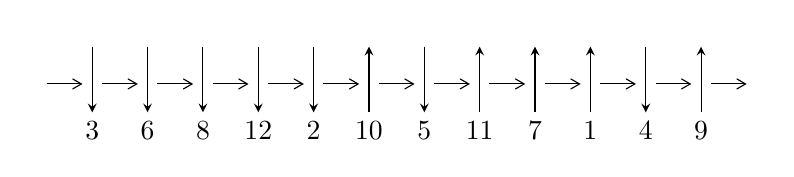
\begin{tikzpicture}[x=20pt, y=17pt]
	% nodes
	\node (C0) at (0, 0) {};
	\node (C1) at (1, 0) {};
	\node (C1U) at (1, +1) {};
	\node (C1D) at (1, -1) {3};

	\node (C2) at (2, 0) {};
	\node (C2U) at (2, +1) {};
	\node (C2D) at (2, -1) {6};

	\node (C3) at (3, 0) {};
	\node (C3U) at (3, +1) {};
	\node (C3D) at (3, -1) {8};

	\node (C4) at (4, 0) {};
	\node (C4U) at (4, +1) {};
	\node (C4D) at (4, -1) {12};

	\node (C5) at (5, 0) {};
	\node (C5U) at (5, +1) {};
	\node (C5D) at (5, -1) {2};

	\node (C6) at (6, 0) {};
	\node (C6U) at (6, +1) {};
	\node (C6D) at (6, -1) {10};

	\node (C7) at (7, 0) {};
	\node (C7U) at (7, +1) {};
	\node (C7D) at (7, -1) {5};

	\node (C8) at (8, 0) {};
	\node (C8U) at (8, +1) {};
	\node (C8D) at (8, -1) {11};

	\node (C9) at (9, 0) {};
	\node (C9U) at (9, +1) {};
	\node (C9D) at (9, -1) {7};

	\node (C10) at (10, 0) {};
	\node (C10U) at (10, +1) {};
	\node (C10D) at (10, -1) {1};

	\node (C11) at (11, 0) {};
	\node (C11U) at (11, +1) {};
	\node (C11D) at (11, -1) {4};

	\node (C12) at (12, 0) {};
	\node (C12U) at (12, +1) {};
	\node (C12D) at (12, -1) {9};
	\node (C13) at (13, 0) {};

	% arrows
	\draw[->,>={angle 60}]
	(C0) edge (C1) (C1) edge (C2) (C2) edge (C3) (C3) edge (C4) (C4) edge (C5) (C5) edge (C6) (C6) edge (C7) (C7) edge (C8) (C8) edge (C9) (C9) edge (C10) (C10) edge (C11) (C11) edge (C12) (C12) edge (C13) ;	\draw[->,>=stealth]
	(C1U) edge (C1D) (C2U) edge (C2D) (C3U) edge (C3D) (C4U) edge (C4D) (C5U) edge (C5D) (C6D) edge (C6U) (C7U) edge (C7D) (C8D) edge (C8U) (C9D) edge (C9U) (C10D) edge (C10U) (C11U) edge (C11D) (C12D) edge (C12U) ;
	\end{tikzpicture} \\
\hhline{~~} \\& 
\textbf{Solving Sequence} \\ \cline{2-2} 
 &
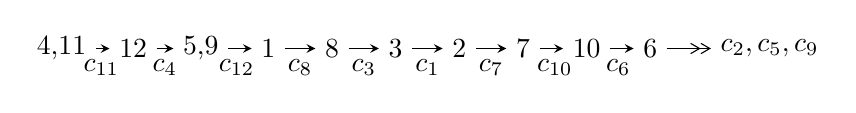
\begin{tikzpicture}[x=23pt, y=7pt]
	% node
	\node (A0) at (-1/8, 0) {4,11};
	\node (A1) at (1, 0) {12};
	\node (A2) at (33/16, 0) {5,9};
	\node (A3) at (25/8, 0) {1};
	\node (A4) at (33/8, 0) {8};
	\node (A5) at (41/8, 0) {3};
	\node (A6) at (49/8, 0) {2};
	\node (A7) at (57/8, 0) {7};
	\node (A8) at (65/8, 0) {10};
	\node (A9) at (73/8, 0) {6};
	\node (C1) at (1/2, -1) {$c_{11}$};
	\node (C2) at (3/2, -1) {$c_{4}$};
	\node (C3) at (21/8, -1) {$c_{12}$};
	\node (C4) at (29/8, -1) {$c_{8}$};
	\node (C5) at (37/8, -1) {$c_{3}$};
	\node (C6) at (45/8, -1) {$c_{1}$};
	\node (C7) at (53/8, -1) {$c_{7}$};
	\node (C8) at (61/8, -1) {$c_{10}$};
	\node (C9) at (69/8, -1) {$c_{6}$};
	\node (A10) at (11, 0) {$c_{2},c_{5},c_{9}$};

	% edge
	\draw[->,>=stealth]	
	(A0) edge (A1) (A1) edge (A2) (A2) edge (A3) (A3) edge (A4) (A4) edge (A5) (A5) edge (A6) (A6) edge (A7) (A7) edge (A8) (A8) edge (A9) ;
	\draw[->>,>={angle 60}]	
	(A9) edge (A10);
\end{tikzpicture} \\ 

\end{tabular} \\

\footnotetext{
The image of knot diagram is generated by the software ``\textbf{Draw programme}" developed by Andrew Bartholomew(\url{http://www.layer8.co.uk/maths/draw/index.htm\#Running-draw}), where we modified some parts for our purpose(\url{https://github.com/CATsTAILs/LinksPainter}).
}\phantom \\ \newline 
\centering \textbf{Ideals for irreducible components\footnotemark of $X_{\text{par}}$} 
 
\begin{align*}
I^u_{1}&=\langle 
-1.34989\times10^{918} u^{181}-3.22581\times10^{917} u^{180}+\cdots+2.21461\times10^{916} b-1.39411\times10^{921},\\
\phantom{I^u_{1}}&\phantom{= \langle  }-2.57960\times10^{921} u^{181}-4.86262\times10^{920} u^{180}+\cdots+1.81819\times10^{919} a-2.49275\times10^{924},\\
\phantom{I^u_{1}}&\phantom{= \langle  }u^{182}+u^{181}+\cdots-206 u+821\rangle \\
I^u_{2}&=\langle 
2.90138\times10^{52} u^{46}+1.98487\times10^{52} u^{45}+\cdots+1.55520\times10^{51} b+1.34305\times10^{53},\\
\phantom{I^u_{2}}&\phantom{= \langle  }1.15009\times10^{54} u^{46}+3.14995\times10^{53} u^{45}+\cdots+1.01088\times10^{53} a+2.16660\times10^{54},\;u^{47}-14 u^{45}+\cdots+22 u-5\rangle \\
\\
\end{align*}
\raggedright * 2 irreducible components of $\dim_{\mathbb{C}}=0$, with total 229 representations.\\
\footnotetext{All coefficients of polynomials are rational numbers. But the coefficients are sometimes approximated in decimal forms when there is not enough margin.}
\newpage
\renewcommand{\arraystretch}{1}
\centering \section*{I. $I^u_{1}= \langle -1.35\times10^{918} u^{181}-3.23\times10^{917} u^{180}+\cdots+2.21\times10^{916} b-1.39\times10^{921},\;-2.58\times10^{921} u^{181}-4.86\times10^{920} u^{180}+\cdots+1.82\times10^{919} a-2.49\times10^{924},\;u^{182}+u^{181}+\cdots-206 u+821 \rangle$}
\flushleft \textbf{(i) Arc colorings}\\
\begin{tabular}{m{7pt} m{180pt} m{7pt} m{180pt} }
\flushright $a_{4}=$&$\begin{pmatrix}0\\u\end{pmatrix}$ \\
\flushright $a_{11}=$&$\begin{pmatrix}1\\0\end{pmatrix}$ \\
\flushright $a_{12}=$&$\begin{pmatrix}1\\u^2\end{pmatrix}$ \\
\flushright $a_{5}=$&$\begin{pmatrix}- u\\- u^3+u\end{pmatrix}$ \\
\flushright $a_{9}=$&$\begin{pmatrix}141.877 u^{181}+26.7442 u^{180}+\cdots-201040. u+137100.\\60.9537 u^{181}+14.5660 u^{180}+\cdots-97088.2 u+62950.8\end{pmatrix}$ \\
\flushright $a_{1}=$&$\begin{pmatrix}120.003 u^{181}+19.8936 u^{180}+\cdots-159392. u+112213.\\71.7888 u^{181}+14.0222 u^{180}+\cdots-108196. u+71970.7\end{pmatrix}$ \\
\flushright $a_{8}=$&$\begin{pmatrix}80.9232 u^{181}+12.1782 u^{180}+\cdots-103952. u+74149.7\\60.9537 u^{181}+14.5660 u^{180}+\cdots-97088.2 u+62950.8\end{pmatrix}$ \\
\flushright $a_{3}=$&$\begin{pmatrix}-84.3228 u^{181}-6.07795 u^{180}+\cdots+96339.5 u-76337.0\\-82.9056 u^{181}-13.0190 u^{180}+\cdots+117637. u-82031.7\end{pmatrix}$ \\
\flushright $a_{2}=$&$\begin{pmatrix}55.6039 u^{181}+6.99742 u^{180}+\cdots-70181.4 u+51777.3\\46.9689 u^{181}+8.17406 u^{180}+\cdots-62154.9 u+41969.3\end{pmatrix}$ \\
\flushright $a_{7}=$&$\begin{pmatrix}133.108 u^{181}+23.5681 u^{180}+\cdots-184287. u+127300.\\40.4958 u^{181}+10.4740 u^{180}+\cdots-68001.0 u+43293.3\end{pmatrix}$ \\
\flushright $a_{10}=$&$\begin{pmatrix}163.280 u^{181}+30.9427 u^{180}+\cdots-239334. u+161713.\\29.0074 u^{181}+6.92794 u^{180}+\cdots-51325.4 u+32705.8\end{pmatrix}$ \\
\flushright $a_{6}=$&$\begin{pmatrix}121.019 u^{181}+24.4340 u^{180}+\cdots-183076. u+122441.\\0.820038 u^{181}+2.02066 u^{180}+\cdots-7688.34 u+4101.54\end{pmatrix}$\\&\end{tabular}
\flushleft \textbf{(ii) Obstruction class $= -1$}\\~\\
\flushleft \textbf{(iii) Cusp Shapes $= 108.123 u^{181}+31.9670 u^{180}+\cdots-230810. u+140442.$}\\~\\
\newpage\renewcommand{\arraystretch}{1}
\flushleft \textbf{(iv) u-Polynomials at the component}\newline \\
\begin{tabular}{m{50pt}|m{274pt}}
Crossings & \hspace{64pt}u-Polynomials at each crossing \\
\hline $$\begin{aligned}c_{1}\end{aligned}$$&$\begin{aligned}
&u^{182}+88 u^{181}+\cdots+1248578 u+100489
\end{aligned}$\\
\hline $$\begin{aligned}c_{2},c_{5}\end{aligned}$$&$\begin{aligned}
&u^{182}+4 u^{181}+\cdots-2136 u-317
\end{aligned}$\\
\hline $$\begin{aligned}c_{3}\end{aligned}$$&$\begin{aligned}
&u^{182}+2 u^{181}+\cdots+9357303 u-1023065
\end{aligned}$\\
\hline $$\begin{aligned}c_{4},c_{11}\end{aligned}$$&$\begin{aligned}
&u^{182}+u^{181}+\cdots-206 u+821
\end{aligned}$\\
\hline $$\begin{aligned}c_{6},c_{9}\end{aligned}$$&$\begin{aligned}
&u^{182}-11 u^{181}+\cdots-271145 u-27293
\end{aligned}$\\
\hline $$\begin{aligned}c_{7}\end{aligned}$$&$\begin{aligned}
&u^{182}-10 u^{181}+\cdots+14736466 u+633233
\end{aligned}$\\
\hline $$\begin{aligned}c_{8}\end{aligned}$$&$\begin{aligned}
&u^{182}+12 u^{181}+\cdots+9037 u+1501
\end{aligned}$\\
\hline $$\begin{aligned}c_{10}\end{aligned}$$&$\begin{aligned}
&u^{182}+18 u^{181}+\cdots-267553107 u-15364313
\end{aligned}$\\
\hline $$\begin{aligned}c_{12}\end{aligned}$$&$\begin{aligned}
&u^{182}-4 u^{181}+\cdots-15899 u-1117
\end{aligned}$\\
\hline
\end{tabular}\\~\\
\newpage\renewcommand{\arraystretch}{1}
\flushleft \textbf{(v) Riley Polynomials at the component}\newline \\
\begin{tabular}{m{50pt}|m{274pt}}
Crossings & \hspace{64pt}Riley Polynomials at each crossing \\
\hline $$\begin{aligned}c_{1}\end{aligned}$$&$\begin{aligned}
&y^{182}+28 y^{181}+\cdots+493256419046 y+10098039121
\end{aligned}$\\
\hline $$\begin{aligned}c_{2},c_{5}\end{aligned}$$&$\begin{aligned}
&y^{182}-88 y^{181}+\cdots-1248578 y+100489
\end{aligned}$\\
\hline $$\begin{aligned}c_{3}\end{aligned}$$&$\begin{aligned}
&y^{182}-24 y^{181}+\cdots-76495395788829 y+1046661994225
\end{aligned}$\\
\hline $$\begin{aligned}c_{4},c_{11}\end{aligned}$$&$\begin{aligned}
&y^{182}-113 y^{181}+\cdots-31772444 y+674041
\end{aligned}$\\
\hline $$\begin{aligned}c_{6},c_{9}\end{aligned}$$&$\begin{aligned}
&y^{182}+103 y^{181}+\cdots+14649934201 y+744907849
\end{aligned}$\\
\hline $$\begin{aligned}c_{7}\end{aligned}$$&$\begin{aligned}
&y^{182}-24 y^{181}+\cdots-93975110617920 y+400984032289
\end{aligned}$\\
\hline $$\begin{aligned}c_{8}\end{aligned}$$&$\begin{aligned}
&y^{182}+28 y^{181}+\cdots-226333749 y+2253001
\end{aligned}$\\
\hline $$\begin{aligned}c_{10}\end{aligned}$$&$\begin{aligned}
&y^{182}+10 y^{181}+\cdots-449099208347609 y+236062113961969
\end{aligned}$\\
\hline $$\begin{aligned}c_{12}\end{aligned}$$&$\begin{aligned}
&y^{182}+38 y^{181}+\cdots-36140519 y+1247689
\end{aligned}$\\
\hline
\end{tabular}\\~\\
\newpage\flushleft \textbf{(vi) Complex Volumes and Cusp Shapes}
$$\begin{array}{c|c|c}  
\text{Solutions to }I^u_{1}& \I (\text{vol} + \sqrt{-1}CS) & \text{Cusp shape}\\
 \hline 
\begin{aligned}
u &= \phantom{-}0.967487 + 0.254898 I \\
a &= -0.30773 + 2.82009 I \\
b &= -0.527290 + 0.418739 I\end{aligned}
 & -3.12735 - 10.86090 I & \phantom{-0.000000 } 0 \\ \hline\begin{aligned}
u &= \phantom{-}0.967487 - 0.254898 I \\
a &= -0.30773 - 2.82009 I \\
b &= -0.527290 - 0.418739 I\end{aligned}
 & -3.12735 + 10.86090 I & \phantom{-0.000000 } 0 \\ \hline\begin{aligned}
u &= -0.972948 + 0.203366 I \\
a &= -0.58964 - 2.90107 I \\
b &= -0.309357 - 0.446463 I\end{aligned}
 & -1.38924 + 5.27013 I & \phantom{-0.000000 } 0 \\ \hline\begin{aligned}
u &= -0.972948 - 0.203366 I \\
a &= -0.58964 + 2.90107 I \\
b &= -0.309357 + 0.446463 I\end{aligned}
 & -1.38924 - 5.27013 I & \phantom{-0.000000 } 0 \\ \hline\begin{aligned}
u &= -0.964022 + 0.232324 I \\
a &= -1.145130 - 0.287648 I \\
b &= -1.94767 - 0.06654 I\end{aligned}
 & -5.72746 + 3.46987 I & \phantom{-0.000000 } 0 \\ \hline\begin{aligned}
u &= -0.964022 - 0.232324 I \\
a &= -1.145130 + 0.287648 I \\
b &= -1.94767 + 0.06654 I\end{aligned}
 & -5.72746 - 3.46987 I & \phantom{-0.000000 } 0 \\ \hline\begin{aligned}
u &= -0.835164 + 0.566635 I \\
a &= \phantom{-}0.644360 - 0.085011 I \\
b &= -0.643442 - 0.474885 I\end{aligned}
 & -0.17421 + 2.27474 I & \phantom{-0.000000 } 0 \\ \hline\begin{aligned}
u &= -0.835164 - 0.566635 I \\
a &= \phantom{-}0.644360 + 0.085011 I \\
b &= -0.643442 + 0.474885 I\end{aligned}
 & -0.17421 - 2.27474 I & \phantom{-0.000000 } 0 \\ \hline\begin{aligned}
u &= -0.087874 + 1.011160 I \\
a &= \phantom{-}0.288761 + 0.253025 I \\
b &= -0.450031 + 0.263768 I\end{aligned}
 & \phantom{-}2.76742 + 1.88734 I & \phantom{-0.000000 } 0 \\ \hline\begin{aligned}
u &= -0.087874 - 1.011160 I \\
a &= \phantom{-}0.288761 - 0.253025 I \\
b &= -0.450031 - 0.263768 I\end{aligned}
 & \phantom{-}2.76742 - 1.88734 I & \phantom{-0.000000 } 0\\
 \hline 
 \end{array}$$\newpage$$\begin{array}{c|c|c}  
\text{Solutions to }I^u_{1}& \I (\text{vol} + \sqrt{-1}CS) & \text{Cusp shape}\\
 \hline 
\begin{aligned}
u &= \phantom{-}0.190909 + 0.964588 I \\
a &= \phantom{-}0.151054 - 0.089980 I \\
b &= \phantom{-}0.766391 + 0.876174 I\end{aligned}
 & \phantom{-}2.70708 + 3.46168 I & \phantom{-0.000000 } 0 \\ \hline\begin{aligned}
u &= \phantom{-}0.190909 - 0.964588 I \\
a &= \phantom{-}0.151054 + 0.089980 I \\
b &= \phantom{-}0.766391 - 0.876174 I\end{aligned}
 & \phantom{-}2.70708 - 3.46168 I & \phantom{-0.000000 } 0 \\ \hline\begin{aligned}
u &= -0.177215 + 0.965718 I \\
a &= \phantom{-}0.127514 + 0.154046 I \\
b &= \phantom{-}0.788455 - 1.005380 I\end{aligned}
 & \phantom{-}0.75906 - 8.61755 I & \phantom{-0.000000 } 0 \\ \hline\begin{aligned}
u &= -0.177215 - 0.965718 I \\
a &= \phantom{-}0.127514 - 0.154046 I \\
b &= \phantom{-}0.788455 + 1.005380 I\end{aligned}
 & \phantom{-}0.75906 + 8.61755 I & \phantom{-0.000000 } 0 \\ \hline\begin{aligned}
u &= -0.188554 + 1.008270 I \\
a &= \phantom{-}0.074830 - 0.279695 I \\
b &= \phantom{-}0.815872 - 0.134276 I\end{aligned}
 & \phantom{-}1.59563 + 4.51296 I & \phantom{-0.000000 } 0 \\ \hline\begin{aligned}
u &= -0.188554 - 1.008270 I \\
a &= \phantom{-}0.074830 + 0.279695 I \\
b &= \phantom{-}0.815872 + 0.134276 I\end{aligned}
 & \phantom{-}1.59563 - 4.51296 I & \phantom{-0.000000 } 0 \\ \hline\begin{aligned}
u &= \phantom{-}0.224357 + 1.008210 I \\
a &= \phantom{-}0.154670 + 0.179447 I \\
b &= \phantom{-}0.702336 + 0.438773 I\end{aligned}
 & \phantom{-}3.07783 + 0.66639 I & \phantom{-0.000000 } 0 \\ \hline\begin{aligned}
u &= \phantom{-}0.224357 - 1.008210 I \\
a &= \phantom{-}0.154670 - 0.179447 I \\
b &= \phantom{-}0.702336 - 0.438773 I\end{aligned}
 & \phantom{-}3.07783 - 0.66639 I & \phantom{-0.000000 } 0 \\ \hline\begin{aligned}
u &= \phantom{-}0.881875 + 0.540906 I \\
a &= \phantom{-}0.776942 - 0.091144 I \\
b &= -0.622106 + 0.509657 I\end{aligned}
 & -1.23669 - 7.22005 I & \phantom{-0.000000 } 0 \\ \hline\begin{aligned}
u &= \phantom{-}0.881875 - 0.540906 I \\
a &= \phantom{-}0.776942 + 0.091144 I \\
b &= -0.622106 - 0.509657 I\end{aligned}
 & -1.23669 + 7.22005 I & \phantom{-0.000000 } 0\\
 \hline 
 \end{array}$$\newpage$$\begin{array}{c|c|c}  
\text{Solutions to }I^u_{1}& \I (\text{vol} + \sqrt{-1}CS) & \text{Cusp shape}\\
 \hline 
\begin{aligned}
u &= -1.018560 + 0.226948 I \\
a &= -1.68765 + 0.38404 I \\
b &= -2.28333 + 0.75686 I\end{aligned}
 & -3.80799 + 10.86370 I & \phantom{-0.000000 } 0 \\ \hline\begin{aligned}
u &= -1.018560 - 0.226948 I \\
a &= -1.68765 - 0.38404 I \\
b &= -2.28333 - 0.75686 I\end{aligned}
 & -3.80799 - 10.86370 I & \phantom{-0.000000 } 0 \\ \hline\begin{aligned}
u &= \phantom{-}1.015510 + 0.251706 I \\
a &= -1.312930 - 0.473605 I \\
b &= -1.86161 - 0.72946 I\end{aligned}
 & -1.59790 - 6.03649 I & \phantom{-0.000000 } 0 \\ \hline\begin{aligned}
u &= \phantom{-}1.015510 - 0.251706 I \\
a &= -1.312930 + 0.473605 I \\
b &= -1.86161 + 0.72946 I\end{aligned}
 & -1.59790 + 6.03649 I & \phantom{-0.000000 } 0 \\ \hline\begin{aligned}
u &= -1.040900 + 0.109055 I \\
a &= -0.81412 - 1.54675 I \\
b &= \phantom{-}0.575716 - 0.826385 I\end{aligned}
 & -2.93164 + 1.40135 I & \phantom{-0.000000 } 0 \\ \hline\begin{aligned}
u &= -1.040900 - 0.109055 I \\
a &= -0.81412 + 1.54675 I \\
b &= \phantom{-}0.575716 + 0.826385 I\end{aligned}
 & -2.93164 - 1.40135 I & \phantom{-0.000000 } 0 \\ \hline\begin{aligned}
u &= -0.181737 + 0.929233 I \\
a &= \phantom{-}0.294651 + 0.173941 I \\
b &= \phantom{-}0.444291 - 0.915303 I\end{aligned}
 & -2.16280 - 1.55039 I & \phantom{-0.000000 } 0 \\ \hline\begin{aligned}
u &= -0.181737 - 0.929233 I \\
a &= \phantom{-}0.294651 - 0.173941 I \\
b &= \phantom{-}0.444291 + 0.915303 I\end{aligned}
 & -2.16280 + 1.55039 I & \phantom{-0.000000 } 0 \\ \hline\begin{aligned}
u &= \phantom{-}1.056600 + 0.082970 I \\
a &= -0.26579 + 1.57419 I \\
b &= \phantom{-}0.90058 + 1.18850 I\end{aligned}
 & -5.51601 + 3.60018 I & \phantom{-0.000000 } 0 \\ \hline\begin{aligned}
u &= \phantom{-}1.056600 - 0.082970 I \\
a &= -0.26579 - 1.57419 I \\
b &= \phantom{-}0.90058 - 1.18850 I\end{aligned}
 & -5.51601 - 3.60018 I & \phantom{-0.000000 } 0\\
 \hline 
 \end{array}$$\newpage$$\begin{array}{c|c|c}  
\text{Solutions to }I^u_{1}& \I (\text{vol} + \sqrt{-1}CS) & \text{Cusp shape}\\
 \hline 
\begin{aligned}
u &= -0.902568 + 0.235395 I \\
a &= -0.555904 + 1.245760 I \\
b &= \phantom{-}1.154090 + 0.195908 I\end{aligned}
 & \phantom{-}1.34326 + 2.98619 I & \phantom{-0.000000 } 0 \\ \hline\begin{aligned}
u &= -0.902568 - 0.235395 I \\
a &= -0.555904 - 1.245760 I \\
b &= \phantom{-}1.154090 - 0.195908 I\end{aligned}
 & \phantom{-}1.34326 - 2.98619 I & \phantom{-0.000000 } 0 \\ \hline\begin{aligned}
u &= \phantom{-}0.966542 + 0.502109 I \\
a &= \phantom{-}0.572313 - 0.569869 I \\
b &= -0.320888 + 0.363036 I\end{aligned}
 & -3.01269 - 2.23958 I & \phantom{-0.000000 } 0 \\ \hline\begin{aligned}
u &= \phantom{-}0.966542 - 0.502109 I \\
a &= \phantom{-}0.572313 + 0.569869 I \\
b &= -0.320888 - 0.363036 I\end{aligned}
 & -3.01269 + 2.23958 I & \phantom{-0.000000 } 0 \\ \hline\begin{aligned}
u &= -0.125474 + 0.902003 I \\
a &= \phantom{-}0.219966 - 0.530351 I \\
b &= \phantom{-}0.727715 + 0.467107 I\end{aligned}
 & -0.526852 - 0.632760 I & \phantom{-0.000000 } 0 \\ \hline\begin{aligned}
u &= -0.125474 - 0.902003 I \\
a &= \phantom{-}0.219966 + 0.530351 I \\
b &= \phantom{-}0.727715 - 0.467107 I\end{aligned}
 & -0.526852 + 0.632760 I & \phantom{-0.000000 } 0 \\ \hline\begin{aligned}
u &= \phantom{-}1.044690 + 0.322840 I \\
a &= -0.595121 - 1.016790 I \\
b &= -0.826001 - 0.963467 I\end{aligned}
 & -0.77669 - 4.47027 I & \phantom{-0.000000 } 0 \\ \hline\begin{aligned}
u &= \phantom{-}1.044690 - 0.322840 I \\
a &= -0.595121 + 1.016790 I \\
b &= -0.826001 + 0.963467 I\end{aligned}
 & -0.77669 + 4.47027 I & \phantom{-0.000000 } 0 \\ \hline\begin{aligned}
u &= -0.904613\phantom{ +0.000000I} \\
a &= \phantom{-}0.111901\phantom{ +0.000000I} \\
b &= \phantom{-}1.33201\phantom{ +0.000000I}\end{aligned}
 & -0.894512\phantom{ +0.000000I} & \phantom{-0.000000 } 0 \\ \hline\begin{aligned}
u &= \phantom{-}1.097740 + 0.153075 I \\
a &= -0.55490 + 2.13977 I \\
b &= -0.092630 + 1.284410 I\end{aligned}
 & -7.74718 - 4.27725 I & \phantom{-0.000000 } 0\\
 \hline 
 \end{array}$$\newpage$$\begin{array}{c|c|c}  
\text{Solutions to }I^u_{1}& \I (\text{vol} + \sqrt{-1}CS) & \text{Cusp shape}\\
 \hline 
\begin{aligned}
u &= \phantom{-}1.097740 - 0.153075 I \\
a &= -0.55490 - 2.13977 I \\
b &= -0.092630 - 1.284410 I\end{aligned}
 & -7.74718 + 4.27725 I & \phantom{-0.000000 } 0 \\ \hline\begin{aligned}
u &= \phantom{-}0.845654 + 0.269944 I \\
a &= -0.50394 - 1.69302 I \\
b &= \phantom{-}1.184740 - 0.161306 I\end{aligned}
 & \phantom{-}0.869585 + 1.087340 I & \phantom{-0.000000 } 0 \\ \hline\begin{aligned}
u &= \phantom{-}0.845654 - 0.269944 I \\
a &= -0.50394 + 1.69302 I \\
b &= \phantom{-}1.184740 + 0.161306 I\end{aligned}
 & \phantom{-}0.869585 - 1.087340 I & \phantom{-0.000000 } 0 \\ \hline\begin{aligned}
u &= -0.686245 + 0.884213 I \\
a &= \phantom{-}0.697850 - 0.543633 I \\
b &= \phantom{-}0.522071 - 0.953460 I\end{aligned}
 & -1.93310 - 3.36486 I & \phantom{-0.000000 } 0 \\ \hline\begin{aligned}
u &= -0.686245 - 0.884213 I \\
a &= \phantom{-}0.697850 + 0.543633 I \\
b &= \phantom{-}0.522071 + 0.953460 I\end{aligned}
 & -1.93310 + 3.36486 I & \phantom{-0.000000 } 0 \\ \hline\begin{aligned}
u &= \phantom{-}0.794036 + 0.346649 I \\
a &= -0.50176 - 2.09286 I \\
b &= \phantom{-}0.266950 - 1.366250 I\end{aligned}
 & \phantom{-}0.63985 - 3.63929 I & \phantom{-0.000000 } 0 \\ \hline\begin{aligned}
u &= \phantom{-}0.794036 - 0.346649 I \\
a &= -0.50176 + 2.09286 I \\
b &= \phantom{-}0.266950 + 1.366250 I\end{aligned}
 & \phantom{-}0.63985 + 3.63929 I & \phantom{-0.000000 } 0 \\ \hline\begin{aligned}
u &= -1.029160 + 0.477949 I \\
a &= \phantom{-}0.404807 + 0.839756 I \\
b &= -0.0919135 - 0.1001910 I\end{aligned}
 & -3.12868 + 5.39424 I & \phantom{-0.000000 } 0 \\ \hline\begin{aligned}
u &= -1.029160 - 0.477949 I \\
a &= \phantom{-}0.404807 - 0.839756 I \\
b &= -0.0919135 + 0.1001910 I\end{aligned}
 & -3.12868 - 5.39424 I & \phantom{-0.000000 } 0 \\ \hline\begin{aligned}
u &= \phantom{-}0.859021 + 0.068455 I \\
a &= \phantom{-}1.28643 + 1.53746 I \\
b &= -0.024971 + 1.198640 I\end{aligned}
 & -4.57409 + 3.98923 I & \phantom{-0.000000 } 0\\
 \hline 
 \end{array}$$\newpage$$\begin{array}{c|c|c}  
\text{Solutions to }I^u_{1}& \I (\text{vol} + \sqrt{-1}CS) & \text{Cusp shape}\\
 \hline 
\begin{aligned}
u &= \phantom{-}0.859021 - 0.068455 I \\
a &= \phantom{-}1.28643 - 1.53746 I \\
b &= -0.024971 - 1.198640 I\end{aligned}
 & -4.57409 - 3.98923 I & \phantom{-0.000000 } 0 \\ \hline\begin{aligned}
u &= -0.828816 + 0.233513 I \\
a &= \phantom{-}1.70869 + 1.06062 I \\
b &= \phantom{-}2.05532 + 0.02976 I\end{aligned}
 & \phantom{-}0.70268 + 3.98023 I & \phantom{-0.000000 } 0 \\ \hline\begin{aligned}
u &= -0.828816 - 0.233513 I \\
a &= \phantom{-}1.70869 - 1.06062 I \\
b &= \phantom{-}2.05532 - 0.02976 I\end{aligned}
 & \phantom{-}0.70268 - 3.98023 I & \phantom{-0.000000 } 0 \\ \hline\begin{aligned}
u &= -1.073330 + 0.389701 I \\
a &= -0.39369 + 1.49829 I \\
b &= -0.128585 + 1.390040 I\end{aligned}
 & -2.42151 + 0.21578 I & \phantom{-0.000000 } 0 \\ \hline\begin{aligned}
u &= -1.073330 - 0.389701 I \\
a &= -0.39369 - 1.49829 I \\
b &= -0.128585 - 1.390040 I\end{aligned}
 & -2.42151 - 0.21578 I & \phantom{-0.000000 } 0 \\ \hline\begin{aligned}
u &= \phantom{-}0.039549 + 1.143810 I \\
a &= \phantom{-}0.113502 - 0.244648 I \\
b &= -0.495855 - 0.488469 I\end{aligned}
 & \phantom{-}3.02568 + 4.10336 I & \phantom{-0.000000 } 0 \\ \hline\begin{aligned}
u &= \phantom{-}0.039549 - 1.143810 I \\
a &= \phantom{-}0.113502 + 0.244648 I \\
b &= -0.495855 + 0.488469 I\end{aligned}
 & \phantom{-}3.02568 - 4.10336 I & \phantom{-0.000000 } 0 \\ \hline\begin{aligned}
u &= -0.830570 + 0.190076 I \\
a &= \phantom{-}1.16119 + 2.45289 I \\
b &= \phantom{-}1.71178 + 1.17409 I\end{aligned}
 & \phantom{-}0.79093 - 1.72256 I & \phantom{-0.000000 } 0 \\ \hline\begin{aligned}
u &= -0.830570 - 0.190076 I \\
a &= \phantom{-}1.16119 - 2.45289 I \\
b &= \phantom{-}1.71178 - 1.17409 I\end{aligned}
 & \phantom{-}0.79093 + 1.72256 I & \phantom{-0.000000 } 0 \\ \hline\begin{aligned}
u &= -1.111580 + 0.293633 I \\
a &= \phantom{-}0.676713 - 0.864211 I \\
b &= -0.132839 - 0.819369 I\end{aligned}
 & -2.18156 + 0.29500 I & \phantom{-0.000000 } 0\\
 \hline 
 \end{array}$$\newpage$$\begin{array}{c|c|c}  
\text{Solutions to }I^u_{1}& \I (\text{vol} + \sqrt{-1}CS) & \text{Cusp shape}\\
 \hline 
\begin{aligned}
u &= -1.111580 - 0.293633 I \\
a &= \phantom{-}0.676713 + 0.864211 I \\
b &= -0.132839 + 0.819369 I\end{aligned}
 & -2.18156 - 0.29500 I & \phantom{-0.000000 } 0 \\ \hline\begin{aligned}
u &= -0.091803 + 1.149840 I \\
a &= -0.152431 + 0.040485 I \\
b &= -0.767848 + 0.977705 I\end{aligned}
 & -2.3826 - 14.7160 I & \phantom{-0.000000 } 0 \\ \hline\begin{aligned}
u &= -0.091803 - 1.149840 I \\
a &= -0.152431 - 0.040485 I \\
b &= -0.767848 - 0.977705 I\end{aligned}
 & -2.3826 + 14.7160 I & \phantom{-0.000000 } 0 \\ \hline\begin{aligned}
u &= -1.130360 + 0.243015 I \\
a &= \phantom{-}0.183032 + 1.263930 I \\
b &= \phantom{-}0.126383 + 0.781885 I\end{aligned}
 & -2.18054 + 0.55221 I & \phantom{-0.000000 } 0 \\ \hline\begin{aligned}
u &= -1.130360 - 0.243015 I \\
a &= \phantom{-}0.183032 - 1.263930 I \\
b &= \phantom{-}0.126383 - 0.781885 I\end{aligned}
 & -2.18054 - 0.55221 I & \phantom{-0.000000 } 0 \\ \hline\begin{aligned}
u &= \phantom{-}0.831880 + 0.140724 I \\
a &= \phantom{-}0.449526 + 1.305320 I \\
b &= -0.86648 + 1.12924 I\end{aligned}
 & -6.01676 - 3.73627 I & \phantom{-0.000000 } 0 \\ \hline\begin{aligned}
u &= \phantom{-}0.831880 - 0.140724 I \\
a &= \phantom{-}0.449526 - 1.305320 I \\
b &= -0.86648 - 1.12924 I\end{aligned}
 & -6.01676 + 3.73627 I & \phantom{-0.000000 } 0 \\ \hline\begin{aligned}
u &= \phantom{-}0.816362 + 0.202099 I \\
a &= \phantom{-}0.45395 - 2.55803 I \\
b &= \phantom{-}1.05437 - 1.31858 I\end{aligned}
 & \phantom{-}2.01808 - 2.50159 I & \phantom{-0.000000 } 0 \\ \hline\begin{aligned}
u &= \phantom{-}0.816362 - 0.202099 I \\
a &= \phantom{-}0.45395 + 2.55803 I \\
b &= \phantom{-}1.05437 + 1.31858 I\end{aligned}
 & \phantom{-}2.01808 + 2.50159 I & \phantom{-0.000000 } 0 \\ \hline\begin{aligned}
u &= \phantom{-}0.091974 + 1.163770 I \\
a &= -0.121939 - 0.091019 I \\
b &= -0.715818 - 0.903719 I\end{aligned}
 & \phantom{-}0.11624 + 8.88617 I & \phantom{-0.000000 } 0\\
 \hline 
 \end{array}$$\newpage$$\begin{array}{c|c|c}  
\text{Solutions to }I^u_{1}& \I (\text{vol} + \sqrt{-1}CS) & \text{Cusp shape}\\
 \hline 
\begin{aligned}
u &= \phantom{-}0.091974 - 1.163770 I \\
a &= -0.121939 + 0.091019 I \\
b &= -0.715818 + 0.903719 I\end{aligned}
 & \phantom{-}0.11624 - 8.88617 I & \phantom{-0.000000 } 0 \\ \hline\begin{aligned}
u &= -0.820782 + 0.032222 I \\
a &= \phantom{-}1.24352 - 1.26259 I \\
b &= -0.288376 - 0.805581 I\end{aligned}
 & -1.97928 + 0.64810 I & \phantom{-0.000000 } 0 \\ \hline\begin{aligned}
u &= -0.820782 - 0.032222 I \\
a &= \phantom{-}1.24352 + 1.26259 I \\
b &= -0.288376 + 0.805581 I\end{aligned}
 & -1.97928 - 0.64810 I & \phantom{-0.000000 } 0 \\ \hline\begin{aligned}
u &= -0.652670 + 0.491541 I \\
a &= -1.10110 + 1.73190 I \\
b &= \phantom{-}0.074773 + 1.411070 I\end{aligned}
 & -2.15560 + 8.39299 I & \phantom{-0.000000 } 0 \\ \hline\begin{aligned}
u &= -0.652670 - 0.491541 I \\
a &= -1.10110 - 1.73190 I \\
b &= \phantom{-}0.074773 - 1.411070 I\end{aligned}
 & -2.15560 - 8.39299 I & \phantom{-0.000000 } 0 \\ \hline\begin{aligned}
u &= -0.123985 + 1.192230 I \\
a &= -0.187716 + 0.214512 I \\
b &= -0.528592 + 0.944275 I\end{aligned}
 & -5.97006 - 5.25269 I & \phantom{-0.000000 } 0 \\ \hline\begin{aligned}
u &= -0.123985 - 1.192230 I \\
a &= -0.187716 - 0.214512 I \\
b &= -0.528592 - 0.944275 I\end{aligned}
 & -5.97006 + 5.25269 I & \phantom{-0.000000 } 0 \\ \hline\begin{aligned}
u &= \phantom{-}1.163770 + 0.287263 I \\
a &= -0.18328 + 2.07475 I \\
b &= -0.86881 + 1.19628 I\end{aligned}
 & -7.39230 - 4.74598 I & \phantom{-0.000000 } 0 \\ \hline\begin{aligned}
u &= \phantom{-}1.163770 - 0.287263 I \\
a &= -0.18328 - 2.07475 I \\
b &= -0.86881 - 1.19628 I\end{aligned}
 & -7.39230 + 4.74598 I & \phantom{-0.000000 } 0 \\ \hline\begin{aligned}
u &= \phantom{-}0.753493 + 0.263496 I \\
a &= \phantom{-}1.339370 - 0.396029 I \\
b &= \phantom{-}1.59112 + 0.32797 I\end{aligned}
 & \phantom{-}2.05563 - 0.00213 I & \phantom{-0.000000 } 0\\
 \hline 
 \end{array}$$\newpage$$\begin{array}{c|c|c}  
\text{Solutions to }I^u_{1}& \I (\text{vol} + \sqrt{-1}CS) & \text{Cusp shape}\\
 \hline 
\begin{aligned}
u &= \phantom{-}0.753493 - 0.263496 I \\
a &= \phantom{-}1.339370 + 0.396029 I \\
b &= \phantom{-}1.59112 - 0.32797 I\end{aligned}
 & \phantom{-}2.05563 + 0.00213 I & \phantom{-0.000000 } 0 \\ \hline\begin{aligned}
u &= \phantom{-}0.107950 + 0.785700 I \\
a &= \phantom{-}0.463913 + 0.664939 I \\
b &= \phantom{-}0.591399 - 0.651827 I\end{aligned}
 & -0.69567 - 2.35740 I & \phantom{-0.000000 } 0 \\ \hline\begin{aligned}
u &= \phantom{-}0.107950 - 0.785700 I \\
a &= \phantom{-}0.463913 - 0.664939 I \\
b &= \phantom{-}0.591399 + 0.651827 I\end{aligned}
 & -0.69567 + 2.35740 I & \phantom{-0.000000 } 0 \\ \hline\begin{aligned}
u &= \phantom{-}0.740181 + 0.211944 I \\
a &= -0.18516 - 2.40295 I \\
b &= \phantom{-}0.869246 + 0.000051 I\end{aligned}
 & \phantom{-}1.24046 - 3.64897 I & \phantom{-0.000000 } 0 \\ \hline\begin{aligned}
u &= \phantom{-}0.740181 - 0.211944 I \\
a &= -0.18516 + 2.40295 I \\
b &= \phantom{-}0.869246 - 0.000051 I\end{aligned}
 & \phantom{-}1.24046 + 3.64897 I & \phantom{-0.000000 } 0 \\ \hline\begin{aligned}
u &= \phantom{-}0.186853 + 0.745839 I \\
a &= \phantom{-}0.570063 - 0.226380 I \\
b &= -0.377541 + 1.061550 I\end{aligned}
 & -4.93131 + 3.00209 I & \phantom{-0.000000 } 0 \\ \hline\begin{aligned}
u &= \phantom{-}0.186853 - 0.745839 I \\
a &= \phantom{-}0.570063 + 0.226380 I \\
b &= -0.377541 - 1.061550 I\end{aligned}
 & -4.93131 - 3.00209 I & \phantom{-0.000000 } 0 \\ \hline\begin{aligned}
u &= -0.756680 + 0.127634 I \\
a &= \phantom{-}0.26849 + 2.59397 I \\
b &= \phantom{-}0.553438 + 0.106524 I\end{aligned}
 & \phantom{-}1.95300 - 0.85678 I & \phantom{-0.000000 } 0 \\ \hline\begin{aligned}
u &= -0.756680 - 0.127634 I \\
a &= \phantom{-}0.26849 - 2.59397 I \\
b &= \phantom{-}0.553438 - 0.106524 I\end{aligned}
 & \phantom{-}1.95300 + 0.85678 I & \phantom{-0.000000 } 0 \\ \hline\begin{aligned}
u &= -0.344323 + 0.660503 I \\
a &= \phantom{-}0.591243 + 0.061273 I \\
b &= -0.487752 - 0.795580 I\end{aligned}
 & -2.28977 + 1.07163 I & \phantom{-0.000000 } 0\\
 \hline 
 \end{array}$$\newpage$$\begin{array}{c|c|c}  
\text{Solutions to }I^u_{1}& \I (\text{vol} + \sqrt{-1}CS) & \text{Cusp shape}\\
 \hline 
\begin{aligned}
u &= -0.344323 - 0.660503 I \\
a &= \phantom{-}0.591243 - 0.061273 I \\
b &= -0.487752 + 0.795580 I\end{aligned}
 & -2.28977 - 1.07163 I & \phantom{-0.000000 } 0 \\ \hline\begin{aligned}
u &= -1.199300 + 0.373122 I \\
a &= \phantom{-}0.19788 - 1.95359 I \\
b &= -1.08041 - 1.28324 I\end{aligned}
 & -9.14257 + 7.70288 I & \phantom{-0.000000 } 0 \\ \hline\begin{aligned}
u &= -1.199300 - 0.373122 I \\
a &= \phantom{-}0.19788 + 1.95359 I \\
b &= -1.08041 + 1.28324 I\end{aligned}
 & -9.14257 - 7.70288 I & \phantom{-0.000000 } 0 \\ \hline\begin{aligned}
u &= \phantom{-}1.079450 + 0.663461 I \\
a &= -0.955256 - 0.403685 I \\
b &= -0.339660 - 0.998737 I\end{aligned}
 & -7.33039 - 0.30758 I & \phantom{-0.000000 } 0 \\ \hline\begin{aligned}
u &= \phantom{-}1.079450 - 0.663461 I \\
a &= -0.955256 + 0.403685 I \\
b &= -0.339660 + 0.998737 I\end{aligned}
 & -7.33039 + 0.30758 I & \phantom{-0.000000 } 0 \\ \hline\begin{aligned}
u &= \phantom{-}1.241750 + 0.253562 I \\
a &= \phantom{-}0.684281 + 0.911896 I \\
b &= -0.006589 + 1.029910 I\end{aligned}
 & -4.23859 + 4.48465 I & \phantom{-0.000000 } 0 \\ \hline\begin{aligned}
u &= \phantom{-}1.241750 - 0.253562 I \\
a &= \phantom{-}0.684281 - 0.911896 I \\
b &= -0.006589 - 1.029910 I\end{aligned}
 & -4.23859 - 4.48465 I & \phantom{-0.000000 } 0 \\ \hline\begin{aligned}
u &= \phantom{-}1.250080 + 0.232396 I \\
a &= -1.14474 - 1.42100 I \\
b &= \phantom{-}0.399400 - 0.722182 I\end{aligned}
 & -7.09566 - 10.38340 I & \phantom{-0.000000 } 0 \\ \hline\begin{aligned}
u &= \phantom{-}1.250080 - 0.232396 I \\
a &= -1.14474 + 1.42100 I \\
b &= \phantom{-}0.399400 + 0.722182 I\end{aligned}
 & -7.09566 + 10.38340 I & \phantom{-0.000000 } 0 \\ \hline\begin{aligned}
u &= -1.265370 + 0.176655 I \\
a &= -0.64177 - 1.82730 I \\
b &= -1.02336 - 1.67538 I\end{aligned}
 & -9.01501 + 2.67631 I & \phantom{-0.000000 } 0\\
 \hline 
 \end{array}$$\newpage$$\begin{array}{c|c|c}  
\text{Solutions to }I^u_{1}& \I (\text{vol} + \sqrt{-1}CS) & \text{Cusp shape}\\
 \hline 
\begin{aligned}
u &= -1.265370 - 0.176655 I \\
a &= -0.64177 + 1.82730 I \\
b &= -1.02336 + 1.67538 I\end{aligned}
 & -9.01501 - 2.67631 I & \phantom{-0.000000 } 0 \\ \hline\begin{aligned}
u &= -1.268980 + 0.150779 I \\
a &= -1.03357 + 1.68922 I \\
b &= \phantom{-}0.270307 + 0.624618 I\end{aligned}
 & -4.47587 + 4.20612 I & \phantom{-0.000000 } 0 \\ \hline\begin{aligned}
u &= -1.268980 - 0.150779 I \\
a &= -1.03357 - 1.68922 I \\
b &= \phantom{-}0.270307 - 0.624618 I\end{aligned}
 & -4.47587 - 4.20612 I & \phantom{-0.000000 } 0 \\ \hline\begin{aligned}
u &= \phantom{-}1.232410 + 0.390277 I \\
a &= \phantom{-}0.522585 + 1.014120 I \\
b &= -0.439523 + 1.066630 I\end{aligned}
 & -6.60849 - 2.65473 I & \phantom{-0.000000 } 0 \\ \hline\begin{aligned}
u &= \phantom{-}1.232410 - 0.390277 I \\
a &= \phantom{-}0.522585 - 1.014120 I \\
b &= -0.439523 - 1.066630 I\end{aligned}
 & -6.60849 + 2.65473 I & \phantom{-0.000000 } 0 \\ \hline\begin{aligned}
u &= \phantom{-}1.258340 + 0.337700 I \\
a &= -0.00392 + 1.63921 I \\
b &= -0.98995 + 1.28321 I\end{aligned}
 & -6.79341 - 4.56023 I & \phantom{-0.000000 } 0 \\ \hline\begin{aligned}
u &= \phantom{-}1.258340 - 0.337700 I \\
a &= -0.00392 - 1.63921 I \\
b &= -0.98995 - 1.28321 I\end{aligned}
 & -6.79341 + 4.56023 I & \phantom{-0.000000 } 0 \\ \hline\begin{aligned}
u &= -1.247690 + 0.386127 I \\
a &= \phantom{-}0.32318 - 1.66360 I \\
b &= -0.95670 - 1.37948 I\end{aligned}
 & -9.09310 + 0.98977 I & \phantom{-0.000000 } 0 \\ \hline\begin{aligned}
u &= -1.247690 - 0.386127 I \\
a &= \phantom{-}0.32318 + 1.66360 I \\
b &= -0.95670 + 1.37948 I\end{aligned}
 & -9.09310 - 0.98977 I & \phantom{-0.000000 } 0 \\ \hline\begin{aligned}
u &= -1.190540 + 0.577083 I \\
a &= \phantom{-}0.330241 - 0.698491 I \\
b &= -0.637800 - 0.621744 I\end{aligned}
 & -0.41051 + 2.49024 I & \phantom{-0.000000 } 0\\
 \hline 
 \end{array}$$\newpage$$\begin{array}{c|c|c}  
\text{Solutions to }I^u_{1}& \I (\text{vol} + \sqrt{-1}CS) & \text{Cusp shape}\\
 \hline 
\begin{aligned}
u &= -1.190540 - 0.577083 I \\
a &= \phantom{-}0.330241 + 0.698491 I \\
b &= -0.637800 + 0.621744 I\end{aligned}
 & -0.41051 - 2.49024 I & \phantom{-0.000000 } 0 \\ \hline\begin{aligned}
u &= \phantom{-}1.201020 + 0.595854 I \\
a &= -0.789266 - 0.964724 I \\
b &= \phantom{-}0.101052 - 1.388490 I\end{aligned}
 & -7.61925 - 8.13804 I & \phantom{-0.000000 } 0 \\ \hline\begin{aligned}
u &= \phantom{-}1.201020 - 0.595854 I \\
a &= -0.789266 + 0.964724 I \\
b &= \phantom{-}0.101052 + 1.388490 I\end{aligned}
 & -7.61925 + 8.13804 I & \phantom{-0.000000 } 0 \\ \hline\begin{aligned}
u &= -1.250390 + 0.505659 I \\
a &= \phantom{-}0.000169 + 1.368790 I \\
b &= \phantom{-}0.534564 + 0.877548 I\end{aligned}
 & -1.70396 + 0.79317 I & \phantom{-0.000000 } 0 \\ \hline\begin{aligned}
u &= -1.250390 - 0.505659 I \\
a &= \phantom{-}0.000169 - 1.368790 I \\
b &= \phantom{-}0.534564 - 0.877548 I\end{aligned}
 & -1.70396 - 0.79317 I & \phantom{-0.000000 } 0 \\ \hline\begin{aligned}
u &= -0.490023 + 0.426406 I \\
a &= -0.62903 - 1.96581 I \\
b &= -0.838322 - 0.462429 I\end{aligned}
 & -4.57982 - 0.64855 I & \phantom{-0.000000 } 0 \\ \hline\begin{aligned}
u &= -0.490023 - 0.426406 I \\
a &= -0.62903 + 1.96581 I \\
b &= -0.838322 + 0.462429 I\end{aligned}
 & -4.57982 + 0.64855 I & \phantom{-0.000000 } 0 \\ \hline\begin{aligned}
u &= \phantom{-}1.243620 + 0.530660 I \\
a &= -0.06973 - 1.50158 I \\
b &= \phantom{-}0.756744 - 1.077000 I\end{aligned}
 & -0.16242 - 6.09615 I & \phantom{-0.000000 } 0 \\ \hline\begin{aligned}
u &= \phantom{-}1.243620 - 0.530660 I \\
a &= -0.06973 + 1.50158 I \\
b &= \phantom{-}0.756744 + 1.077000 I\end{aligned}
 & -0.16242 + 6.09615 I & \phantom{-0.000000 } 0 \\ \hline\begin{aligned}
u &= \phantom{-}1.327170 + 0.274433 I \\
a &= -0.38436 + 1.45530 I \\
b &= -1.15380 + 1.30447 I\end{aligned}
 & -6.32752 - 4.77261 I & \phantom{-0.000000 } 0\\
 \hline 
 \end{array}$$\newpage$$\begin{array}{c|c|c}  
\text{Solutions to }I^u_{1}& \I (\text{vol} + \sqrt{-1}CS) & \text{Cusp shape}\\
 \hline 
\begin{aligned}
u &= \phantom{-}1.327170 - 0.274433 I \\
a &= -0.38436 - 1.45530 I \\
b &= -1.15380 - 1.30447 I\end{aligned}
 & -6.32752 + 4.77261 I & \phantom{-0.000000 } 0 \\ \hline\begin{aligned}
u &= \phantom{-}1.250580 + 0.544743 I \\
a &= -0.20568 - 1.64799 I \\
b &= \phantom{-}0.98355 - 1.32703 I\end{aligned}
 & -0.60284 - 8.89547 I & \phantom{-0.000000 } 0 \\ \hline\begin{aligned}
u &= \phantom{-}1.250580 - 0.544743 I \\
a &= -0.20568 + 1.64799 I \\
b &= \phantom{-}0.98355 + 1.32703 I\end{aligned}
 & -0.60284 + 8.89547 I & \phantom{-0.000000 } 0 \\ \hline\begin{aligned}
u &= -1.348520 + 0.212276 I \\
a &= -0.64362 - 1.46962 I \\
b &= -1.30906 - 1.44394 I\end{aligned}
 & -7.90985 + 9.00865 I & \phantom{-0.000000 } 0 \\ \hline\begin{aligned}
u &= -1.348520 - 0.212276 I \\
a &= -0.64362 + 1.46962 I \\
b &= -1.30906 + 1.44394 I\end{aligned}
 & -7.90985 - 9.00865 I & \phantom{-0.000000 } 0 \\ \hline\begin{aligned}
u &= -1.252690 + 0.547183 I \\
a &= -0.25567 + 1.70519 I \\
b &= \phantom{-}1.04603 + 1.41864 I\end{aligned}
 & -2.5811 + 14.0617 I & \phantom{-0.000000 } 0 \\ \hline\begin{aligned}
u &= -1.252690 - 0.547183 I \\
a &= -0.25567 - 1.70519 I \\
b &= \phantom{-}1.04603 - 1.41864 I\end{aligned}
 & -2.5811 - 14.0617 I & \phantom{-0.000000 } 0 \\ \hline\begin{aligned}
u &= -1.258110 + 0.545589 I \\
a &= -0.33758 + 1.48795 I \\
b &= \phantom{-}0.76343 + 1.44186 I\end{aligned}
 & -5.49882 + 6.94092 I & \phantom{-0.000000 } 0 \\ \hline\begin{aligned}
u &= -1.258110 - 0.545589 I \\
a &= -0.33758 - 1.48795 I \\
b &= \phantom{-}0.76343 - 1.44186 I\end{aligned}
 & -5.49882 - 6.94092 I & \phantom{-0.000000 } 0 \\ \hline\begin{aligned}
u &= -0.563917 + 0.234469 I \\
a &= \phantom{-}1.396420 + 0.070335 I \\
b &= -0.902138 + 0.405808 I\end{aligned}
 & -0.36641 - 3.02530 I & \phantom{-0.000000 } 0\\
 \hline 
 \end{array}$$\newpage$$\begin{array}{c|c|c}  
\text{Solutions to }I^u_{1}& \I (\text{vol} + \sqrt{-1}CS) & \text{Cusp shape}\\
 \hline 
\begin{aligned}
u &= -0.563917 - 0.234469 I \\
a &= \phantom{-}1.396420 - 0.070335 I \\
b &= -0.902138 - 0.405808 I\end{aligned}
 & -0.36641 + 3.02530 I & \phantom{-0.000000 } 0 \\ \hline\begin{aligned}
u &= -1.302430 + 0.497353 I \\
a &= \phantom{-}0.002203 + 1.382010 I \\
b &= \phantom{-}0.82900 + 1.38995 I\end{aligned}
 & -4.76193 + 7.14291 I & \phantom{-0.000000 } 0 \\ \hline\begin{aligned}
u &= -1.302430 - 0.497353 I \\
a &= \phantom{-}0.002203 - 1.382010 I \\
b &= \phantom{-}0.82900 - 1.38995 I\end{aligned}
 & -4.76193 - 7.14291 I & \phantom{-0.000000 } 0 \\ \hline\begin{aligned}
u &= -1.206260 + 0.703503 I \\
a &= -0.575121 + 0.588176 I \\
b &= \phantom{-}0.070606 + 0.951096 I\end{aligned}
 & -4.26061 + 4.53255 I & \phantom{-0.000000 } 0 \\ \hline\begin{aligned}
u &= -1.206260 - 0.703503 I \\
a &= -0.575121 - 0.588176 I \\
b &= \phantom{-}0.070606 - 0.951096 I\end{aligned}
 & -4.26061 - 4.53255 I & \phantom{-0.000000 } 0 \\ \hline\begin{aligned}
u &= \phantom{-}0.499712 + 0.328573 I \\
a &= \phantom{-}1.346910 + 0.056551 I \\
b &= -1.064240 - 0.432848 I\end{aligned}
 & -1.92088 + 8.14717 I & \phantom{-0.000000 } 0 \\ \hline\begin{aligned}
u &= \phantom{-}0.499712 - 0.328573 I \\
a &= \phantom{-}1.346910 - 0.056551 I \\
b &= -1.064240 + 0.432848 I\end{aligned}
 & -1.92088 - 8.14717 I & \phantom{-0.000000 } 0 \\ \hline\begin{aligned}
u &= \phantom{-}1.279260 + 0.585636 I \\
a &= \phantom{-}0.212322 + 0.711208 I \\
b &= -0.771852 + 0.657770 I\end{aligned}
 & -1.36807 - 7.95981 I & \phantom{-0.000000 } 0 \\ \hline\begin{aligned}
u &= \phantom{-}1.279260 - 0.585636 I \\
a &= \phantom{-}0.212322 - 0.711208 I \\
b &= -0.771852 - 0.657770 I\end{aligned}
 & -1.36807 + 7.95981 I & \phantom{-0.000000 } 0 \\ \hline\begin{aligned}
u &= \phantom{-}0.458083 + 0.375316 I \\
a &= \phantom{-}1.014560 + 0.017135 I \\
b &= \phantom{-}0.933547 + 0.428630 I\end{aligned}
 & \phantom{-}1.48452 + 0.24598 I & \phantom{-0.000000 } 0\\
 \hline 
 \end{array}$$\newpage$$\begin{array}{c|c|c}  
\text{Solutions to }I^u_{1}& \I (\text{vol} + \sqrt{-1}CS) & \text{Cusp shape}\\
 \hline 
\begin{aligned}
u &= \phantom{-}0.458083 - 0.375316 I \\
a &= \phantom{-}1.014560 - 0.017135 I \\
b &= \phantom{-}0.933547 - 0.428630 I\end{aligned}
 & \phantom{-}1.48452 - 0.24598 I & \phantom{-0.000000 } 0 \\ \hline\begin{aligned}
u &= -1.35920 + 0.46098 I \\
a &= \phantom{-}0.33236 - 1.40819 I \\
b &= -0.478055 - 0.796358 I\end{aligned}
 & -1.33627 + 3.25688 I & \phantom{-0.000000 } 0 \\ \hline\begin{aligned}
u &= -1.35920 - 0.46098 I \\
a &= \phantom{-}0.33236 + 1.40819 I \\
b &= -0.478055 + 0.796358 I\end{aligned}
 & -1.33627 - 3.25688 I & \phantom{-0.000000 } 0 \\ \hline\begin{aligned}
u &= \phantom{-}0.137136 + 0.522429 I \\
a &= \phantom{-}1.35737 + 0.93214 I \\
b &= \phantom{-}0.236107 - 0.701864 I\end{aligned}
 & \phantom{-}0.66176 + 3.13185 I & \phantom{-0.000000 } 0 \\ \hline\begin{aligned}
u &= \phantom{-}0.137136 - 0.522429 I \\
a &= \phantom{-}1.35737 - 0.93214 I \\
b &= \phantom{-}0.236107 + 0.701864 I\end{aligned}
 & \phantom{-}0.66176 - 3.13185 I & \phantom{-0.000000 } 0 \\ \hline\begin{aligned}
u &= \phantom{-}1.35284 + 0.54975 I \\
a &= \phantom{-}0.239246 + 1.386270 I \\
b &= -0.680725 + 0.959726 I\end{aligned}
 & -1.11529 - 9.99689 I & \phantom{-0.000000 } 0 \\ \hline\begin{aligned}
u &= \phantom{-}1.35284 - 0.54975 I \\
a &= \phantom{-}0.239246 - 1.386270 I \\
b &= -0.680725 - 0.959726 I\end{aligned}
 & -1.11529 + 9.99689 I & \phantom{-0.000000 } 0 \\ \hline\begin{aligned}
u &= \phantom{-}0.090290 + 0.531560 I \\
a &= \phantom{-}0.809875 - 0.180341 I \\
b &= -0.761436 + 0.989699 I\end{aligned}
 & -5.52094 - 4.14895 I & \phantom{-0.000000 } 0 \\ \hline\begin{aligned}
u &= \phantom{-}0.090290 - 0.531560 I \\
a &= \phantom{-}0.809875 + 0.180341 I \\
b &= -0.761436 - 0.989699 I\end{aligned}
 & -5.52094 + 4.14895 I & \phantom{-0.000000 } 0 \\ \hline\begin{aligned}
u &= \phantom{-}1.37301 + 0.50046 I \\
a &= \phantom{-}0.236119 - 1.185890 I \\
b &= \phantom{-}1.08257 - 1.15709 I\end{aligned}
 & -5.11354 - 4.53270 I & \phantom{-0.000000 } 0\\
 \hline 
 \end{array}$$\newpage$$\begin{array}{c|c|c}  
\text{Solutions to }I^u_{1}& \I (\text{vol} + \sqrt{-1}CS) & \text{Cusp shape}\\
 \hline 
\begin{aligned}
u &= \phantom{-}1.37301 - 0.50046 I \\
a &= \phantom{-}0.236119 + 1.185890 I \\
b &= \phantom{-}1.08257 + 1.15709 I\end{aligned}
 & -5.11354 + 4.53270 I & \phantom{-0.000000 } 0 \\ \hline\begin{aligned}
u &= -1.34145 + 0.58069 I \\
a &= \phantom{-}0.15394 - 1.61859 I \\
b &= -1.01784 - 1.39051 I\end{aligned}
 & -6.3143 + 20.7901 I & \phantom{-0.000000 } 0 \\ \hline\begin{aligned}
u &= -1.34145 - 0.58069 I \\
a &= \phantom{-}0.15394 + 1.61859 I \\
b &= -1.01784 + 1.39051 I\end{aligned}
 & -6.3143 - 20.7901 I & \phantom{-0.000000 } 0 \\ \hline\begin{aligned}
u &= \phantom{-}1.34340 + 0.58186 I \\
a &= \phantom{-}0.16385 + 1.56913 I \\
b &= -0.95738 + 1.31261 I\end{aligned}
 & -3.8297 - 14.9948 I & \phantom{-0.000000 } 0 \\ \hline\begin{aligned}
u &= \phantom{-}1.34340 - 0.58186 I \\
a &= \phantom{-}0.16385 - 1.56913 I \\
b &= -0.95738 - 1.31261 I\end{aligned}
 & -3.8297 + 14.9948 I & \phantom{-0.000000 } 0 \\ \hline\begin{aligned}
u &= -1.34658 + 0.59072 I \\
a &= \phantom{-}0.25884 - 1.54502 I \\
b &= -0.75965 - 1.35910 I\end{aligned}
 & -9.8712 + 11.4792 I & \phantom{-0.000000 } 0 \\ \hline\begin{aligned}
u &= -1.34658 - 0.59072 I \\
a &= \phantom{-}0.25884 + 1.54502 I \\
b &= -0.75965 + 1.35910 I\end{aligned}
 & -9.8712 - 11.4792 I & \phantom{-0.000000 } 0 \\ \hline\begin{aligned}
u &= -0.00527 + 1.48621 I \\
a &= \phantom{-}0.102694 + 0.138749 I \\
b &= \phantom{-}0.008483 - 0.159656 I\end{aligned}
 & \phantom{-}2.73298 + 1.48892 I & \phantom{-0.000000 } 0 \\ \hline\begin{aligned}
u &= -0.00527 - 1.48621 I \\
a &= \phantom{-}0.102694 - 0.138749 I \\
b &= \phantom{-}0.008483 + 0.159656 I\end{aligned}
 & \phantom{-}2.73298 - 1.48892 I & \phantom{-0.000000 } 0 \\ \hline\begin{aligned}
u &= \phantom{-}1.47579 + 0.28984 I \\
a &= -0.549226 - 1.063220 I \\
b &= \phantom{-}0.109329 - 0.862747 I\end{aligned}
 & -11.80630 - 0.40330 I & \phantom{-0.000000 } 0\\
 \hline 
 \end{array}$$\newpage$$\begin{array}{c|c|c}  
\text{Solutions to }I^u_{1}& \I (\text{vol} + \sqrt{-1}CS) & \text{Cusp shape}\\
 \hline 
\begin{aligned}
u &= \phantom{-}1.47579 - 0.28984 I \\
a &= -0.549226 + 1.063220 I \\
b &= \phantom{-}0.109329 + 0.862747 I\end{aligned}
 & -11.80630 + 0.40330 I & \phantom{-0.000000 } 0 \\ \hline\begin{aligned}
u &= -0.464602 + 0.150603 I \\
a &= -1.16388 - 3.54937 I \\
b &= -0.766226 - 1.151040 I\end{aligned}
 & -2.28151 - 8.69540 I & \phantom{-0.000000 -}0. + 4.30114 I \\ \hline\begin{aligned}
u &= -0.464602 - 0.150603 I \\
a &= -1.16388 + 3.54937 I \\
b &= -0.766226 + 1.151040 I\end{aligned}
 & -2.28151 + 8.69540 I & \phantom{-0.000000 } 0. - 4.30114 I \\ \hline\begin{aligned}
u &= -0.40847 + 1.49083 I \\
a &= -0.019917 - 0.175940 I \\
b &= -0.0426896 + 0.1019610 I\end{aligned}
 & \phantom{-}2.46139 + 4.34383 I & \phantom{-0.000000 } 0 \\ \hline\begin{aligned}
u &= -0.40847 - 1.49083 I \\
a &= -0.019917 + 0.175940 I \\
b &= -0.0426896 - 0.1019610 I\end{aligned}
 & \phantom{-}2.46139 - 4.34383 I & \phantom{-0.000000 } 0 \\ \hline\begin{aligned}
u &= \phantom{-}1.45120 + 0.54244 I \\
a &= \phantom{-}0.321634 - 0.816869 I \\
b &= \phantom{-}1.046230 - 0.694732 I\end{aligned}
 & -3.60511 - 10.20840 I & \phantom{-0.000000 } 0 \\ \hline\begin{aligned}
u &= \phantom{-}1.45120 - 0.54244 I \\
a &= \phantom{-}0.321634 + 0.816869 I \\
b &= \phantom{-}1.046230 + 0.694732 I\end{aligned}
 & -3.60511 + 10.20840 I & \phantom{-0.000000 } 0 \\ \hline\begin{aligned}
u &= -0.443920\phantom{ +0.000000I} \\
a &= \phantom{-}1.06128\phantom{ +0.000000I} \\
b &= \phantom{-}0.0546188\phantom{ +0.000000I}\end{aligned}
 & -0.910151\phantom{ +0.000000I} & -11.4070\phantom{ +0.000000I} \\ \hline\begin{aligned}
u &= -1.44146 + 0.60882 I \\
a &= \phantom{-}0.127731 + 0.715132 I \\
b &= \phantom{-}0.781262 + 0.679976 I\end{aligned}
 & -2.31935 + 5.53454 I & \phantom{-0.000000 } 0 \\ \hline\begin{aligned}
u &= -1.44146 - 0.60882 I \\
a &= \phantom{-}0.127731 - 0.715132 I \\
b &= \phantom{-}0.781262 - 0.679976 I\end{aligned}
 & -2.31935 - 5.53454 I & \phantom{-0.000000 } 0\\
 \hline 
 \end{array}$$\newpage$$\begin{array}{c|c|c}  
\text{Solutions to }I^u_{1}& \I (\text{vol} + \sqrt{-1}CS) & \text{Cusp shape}\\
 \hline 
\begin{aligned}
u &= -1.53405 + 0.33866 I \\
a &= -0.394386 + 0.735351 I \\
b &= \phantom{-}0.039617 + 0.817119 I\end{aligned}
 & -5.43574 - 2.99336 I & \phantom{-0.000000 } 0 \\ \hline\begin{aligned}
u &= -1.53405 - 0.33866 I \\
a &= -0.394386 - 0.735351 I \\
b &= \phantom{-}0.039617 - 0.817119 I\end{aligned}
 & -5.43574 + 2.99336 I & \phantom{-0.000000 } 0 \\ \hline\begin{aligned}
u &= \phantom{-}1.53169 + 0.37881 I \\
a &= -0.504272 - 0.638100 I \\
b &= -0.016873 - 0.840689 I\end{aligned}
 & -7.77632 + 8.84108 I & \phantom{-0.000000 } 0 \\ \hline\begin{aligned}
u &= \phantom{-}1.53169 - 0.37881 I \\
a &= -0.504272 + 0.638100 I \\
b &= -0.016873 + 0.840689 I\end{aligned}
 & -7.77632 - 8.84108 I & \phantom{-0.000000 } 0 \\ \hline\begin{aligned}
u &= -0.045591 + 0.419352 I \\
a &= \phantom{-}2.06623 - 0.13714 I \\
b &= \phantom{-}0.041357 + 0.585616 I\end{aligned}
 & \phantom{-}1.84649 + 1.49859 I & \phantom{-}1.71665 - 3.18263 I \\ \hline\begin{aligned}
u &= -0.045591 - 0.419352 I \\
a &= \phantom{-}2.06623 + 0.13714 I \\
b &= \phantom{-}0.041357 - 0.585616 I\end{aligned}
 & \phantom{-}1.84649 - 1.49859 I & \phantom{-}1.71665 + 3.18263 I \\ \hline\begin{aligned}
u &= \phantom{-}0.340065 + 0.227248 I \\
a &= -0.06323 + 3.57673 I \\
b &= -0.555145 + 0.892699 I\end{aligned}
 & \phantom{-}0.13863 + 3.60138 I & \phantom{-}0.707136 - 1.018842 I \\ \hline\begin{aligned}
u &= \phantom{-}0.340065 - 0.227248 I \\
a &= -0.06323 - 3.57673 I \\
b &= -0.555145 - 0.892699 I\end{aligned}
 & \phantom{-}0.13863 - 3.60138 I & \phantom{-}0.707136 + 1.018842 I \\ \hline\begin{aligned}
u &= \phantom{-}0.192999 + 0.295018 I \\
a &= \phantom{-}1.077820 + 0.093282 I \\
b &= -0.992207 - 0.758059 I\end{aligned}
 & -4.55239 + 2.14279 I & \phantom{-}0.84674 + 3.42738 I \\ \hline\begin{aligned}
u &= \phantom{-}0.192999 - 0.295018 I \\
a &= \phantom{-}1.077820 - 0.093282 I \\
b &= -0.992207 + 0.758059 I\end{aligned}
 & -4.55239 - 2.14279 I & \phantom{-}0.84674 - 3.42738 I\\
 \hline 
 \end{array}$$\newpage$$\begin{array}{c|c|c}  
\text{Solutions to }I^u_{1}& \I (\text{vol} + \sqrt{-1}CS) & \text{Cusp shape}\\
 \hline 
\begin{aligned}
u &= \phantom{-}1.65412 + 0.03387 I \\
a &= -0.169939 - 1.396720 I \\
b &= -0.002160 - 0.831633 I\end{aligned}
 & -11.87070 - 0.00423 I & \phantom{-0.000000 } 0 \\ \hline\begin{aligned}
u &= \phantom{-}1.65412 - 0.03387 I \\
a &= -0.169939 + 1.396720 I \\
b &= -0.002160 + 0.831633 I\end{aligned}
 & -11.87070 + 0.00423 I & \phantom{-0.000000 } 0\\
 \hline 
 \end{array}$$\newpage\newpage\renewcommand{\arraystretch}{1}
\centering \section*{II. $I^u_{2}= \langle 2.90\times10^{52} u^{46}+1.98\times10^{52} u^{45}+\cdots+1.56\times10^{51} b+1.34\times10^{53},\;1.15\times10^{54} u^{46}+3.15\times10^{53} u^{45}+\cdots+1.01\times10^{53} a+2.17\times10^{54},\;u^{47}-14 u^{45}+\cdots+22 u-5 \rangle$}
\flushleft \textbf{(i) Arc colorings}\\
\begin{tabular}{m{7pt} m{180pt} m{7pt} m{180pt} }
\flushright $a_{4}=$&$\begin{pmatrix}0\\u\end{pmatrix}$ \\
\flushright $a_{11}=$&$\begin{pmatrix}1\\0\end{pmatrix}$ \\
\flushright $a_{12}=$&$\begin{pmatrix}1\\u^2\end{pmatrix}$ \\
\flushright $a_{5}=$&$\begin{pmatrix}- u\\- u^3+u\end{pmatrix}$ \\
\flushright $a_{9}=$&$\begin{pmatrix}-11.3772 u^{46}-3.11604 u^{45}+\cdots+12.7802 u-21.4328\\-18.6560 u^{46}-12.7628 u^{45}+\cdots+276.348 u-86.3588\end{pmatrix}$ \\
\flushright $a_{1}=$&$\begin{pmatrix}-4.43668 u^{46}+0.763475 u^{45}+\cdots+111.108 u-38.3966\\1.70932 u^{46}-4.54241 u^{45}+\cdots+108.873 u-15.0617\end{pmatrix}$ \\
\flushright $a_{8}=$&$\begin{pmatrix}7.27883 u^{46}+9.64675 u^{45}+\cdots-263.568 u+64.9260\\-18.6560 u^{46}-12.7628 u^{45}+\cdots+276.348 u-86.3588\end{pmatrix}$ \\
\flushright $a_{3}=$&$\begin{pmatrix}2.71300 u^{46}+5.20585 u^{45}+\cdots+72.2141 u-27.8985\\0.791965 u^{46}+7.72928 u^{45}+\cdots-376.925 u+95.4057\end{pmatrix}$ \\
\flushright $a_{2}=$&$\begin{pmatrix}21.8719 u^{46}+1.26403 u^{45}+\cdots+84.7675 u+20.1723\\-2.68860 u^{46}-0.337691 u^{45}+\cdots-95.9220 u+24.6307\end{pmatrix}$ \\
\flushright $a_{7}=$&$\begin{pmatrix}-4.43230 u^{46}+4.59548 u^{45}+\cdots-148.787 u+19.5765\\-14.3067 u^{46}-9.75470 u^{45}+\cdots+214.139 u-66.2657\end{pmatrix}$ \\
\flushright $a_{10}=$&$\begin{pmatrix}5.21616 u^{46}+12.4608 u^{45}+\cdots-355.423 u+80.1633\\-6.63107 u^{46}+2.48523 u^{45}+\cdots-97.2484 u+5.58692\end{pmatrix}$ \\
\flushright $a_{6}=$&$\begin{pmatrix}21.3283 u^{46}-1.97448 u^{45}+\cdots+40.9224 u+35.5953\\-1.12322 u^{46}-4.68109 u^{45}+\cdots+90.5828 u-18.9323\end{pmatrix}$\\&\end{tabular}
\flushleft \textbf{(ii) Obstruction class $= 1$}\\~\\
\flushleft \textbf{(iii) Cusp Shapes $= 31.3541 u^{46}-23.9200 u^{45}+\cdots+698.106 u-92.0366$}\\~\\
\newpage\renewcommand{\arraystretch}{1}
\flushleft \textbf{(iv) u-Polynomials at the component}\newline \\
\begin{tabular}{m{50pt}|m{274pt}}
Crossings & \hspace{64pt}u-Polynomials at each crossing \\
\hline $$\begin{aligned}c_{1}\end{aligned}$$&$\begin{aligned}
&u^{47}-27 u^{46}+\cdots+34 u-1
\end{aligned}$\\
\hline $$\begin{aligned}c_{2}\end{aligned}$$&$\begin{aligned}
&u^{47}+3 u^{46}+\cdots+4 u-1
\end{aligned}$\\
\hline $$\begin{aligned}c_{3}\end{aligned}$$&$\begin{aligned}
&u^{47}+u^{46}+\cdots+5 u-1
\end{aligned}$\\
\hline $$\begin{aligned}c_{4}\end{aligned}$$&$\begin{aligned}
&u^{47}-14 u^{45}+\cdots+22 u+5
\end{aligned}$\\
\hline $$\begin{aligned}c_{5}\end{aligned}$$&$\begin{aligned}
&u^{47}-3 u^{46}+\cdots+4 u+1
\end{aligned}$\\
\hline $$\begin{aligned}c_{6}\end{aligned}$$&$\begin{aligned}
&u^{47}+18 u^{46}+\cdots+73 u+5
\end{aligned}$\\
\hline $$\begin{aligned}c_{7}\end{aligned}$$&$\begin{aligned}
&u^{47}+3 u^{46}+\cdots-18 u+5
\end{aligned}$\\
\hline $$\begin{aligned}c_{8}\end{aligned}$$&$\begin{aligned}
&u^{47}+5 u^{46}+\cdots+3 u+1
\end{aligned}$\\
\hline $$\begin{aligned}c_{9}\end{aligned}$$&$\begin{aligned}
&u^{47}-18 u^{46}+\cdots+73 u-5
\end{aligned}$\\
\hline $$\begin{aligned}c_{10}\end{aligned}$$&$\begin{aligned}
&u^{47}+u^{46}+\cdots-33 u+5
\end{aligned}$\\
\hline $$\begin{aligned}c_{11}\end{aligned}$$&$\begin{aligned}
&u^{47}-14 u^{45}+\cdots+22 u-5
\end{aligned}$\\
\hline $$\begin{aligned}c_{12}\end{aligned}$$&$\begin{aligned}
&u^{47}+3 u^{46}+\cdots+7 u-1
\end{aligned}$\\
\hline
\end{tabular}\\~\\
\newpage\renewcommand{\arraystretch}{1}
\flushleft \textbf{(v) Riley Polynomials at the component}\newline \\
\begin{tabular}{m{50pt}|m{274pt}}
Crossings & \hspace{64pt}Riley Polynomials at each crossing \\
\hline $$\begin{aligned}c_{1}\end{aligned}$$&$\begin{aligned}
&y^{47}+y^{46}+\cdots+62 y-1
\end{aligned}$\\
\hline $$\begin{aligned}c_{2},c_{5}\end{aligned}$$&$\begin{aligned}
&y^{47}-27 y^{46}+\cdots+34 y-1
\end{aligned}$\\
\hline $$\begin{aligned}c_{3}\end{aligned}$$&$\begin{aligned}
&y^{47}+13 y^{46}+\cdots+29 y-1
\end{aligned}$\\
\hline $$\begin{aligned}c_{4},c_{11}\end{aligned}$$&$\begin{aligned}
&y^{47}-28 y^{46}+\cdots+604 y-25
\end{aligned}$\\
\hline $$\begin{aligned}c_{6},c_{9}\end{aligned}$$&$\begin{aligned}
&y^{47}+24 y^{46}+\cdots-521 y-25
\end{aligned}$\\
\hline $$\begin{aligned}c_{7}\end{aligned}$$&$\begin{aligned}
&y^{47}-23 y^{46}+\cdots+344 y-25
\end{aligned}$\\
\hline $$\begin{aligned}c_{8}\end{aligned}$$&$\begin{aligned}
&y^{47}-11 y^{46}+\cdots-7 y-1
\end{aligned}$\\
\hline $$\begin{aligned}c_{10}\end{aligned}$$&$\begin{aligned}
&y^{47}-21 y^{46}+\cdots+69 y-25
\end{aligned}$\\
\hline $$\begin{aligned}c_{12}\end{aligned}$$&$\begin{aligned}
&y^{47}+27 y^{46}+\cdots-5 y-1
\end{aligned}$\\
\hline
\end{tabular}\\~\\
\newpage\flushleft \textbf{(vi) Complex Volumes and Cusp Shapes}
$$\begin{array}{c|c|c}  
\text{Solutions to }I^u_{2}& \I (\text{vol} + \sqrt{-1}CS) & \text{Cusp shape}\\
 \hline 
\begin{aligned}
u &= \phantom{-}0.464174 + 0.870325 I \\
a &= \phantom{-}0.943277 + 0.252341 I \\
b &= \phantom{-}0.520750 + 0.880085 I\end{aligned}
 & -2.34055 + 2.89236 I & -9.31056 + 0. I\phantom{ +0.000000I} \\ \hline\begin{aligned}
u &= \phantom{-}0.464174 - 0.870325 I \\
a &= \phantom{-}0.943277 - 0.252341 I \\
b &= \phantom{-}0.520750 - 0.880085 I\end{aligned}
 & -2.34055 - 2.89236 I & -9.31056 + 0. I\phantom{ +0.000000I} \\ \hline\begin{aligned}
u &= -0.908286 + 0.225806 I \\
a &= \phantom{-}0.93278 + 1.40918 I \\
b &= \phantom{-}1.61302 + 0.08073 I\end{aligned}
 & \phantom{-}0.10624 + 3.79429 I & -11.66811 - 6.10729 I \\ \hline\begin{aligned}
u &= -0.908286 - 0.225806 I \\
a &= \phantom{-}0.93278 - 1.40918 I \\
b &= \phantom{-}1.61302 - 0.08073 I\end{aligned}
 & \phantom{-}0.10624 - 3.79429 I & -11.66811 + 6.10729 I \\ \hline\begin{aligned}
u &= \phantom{-}0.851476 + 0.294853 I \\
a &= \phantom{-}0.342248 - 1.087160 I \\
b &= \phantom{-}1.180730 + 0.029589 I\end{aligned}
 & \phantom{-}1.090700 - 0.120524 I & -3.56317 + 4.82730 I \\ \hline\begin{aligned}
u &= \phantom{-}0.851476 - 0.294853 I \\
a &= \phantom{-}0.342248 + 1.087160 I \\
b &= \phantom{-}1.180730 - 0.029589 I\end{aligned}
 & \phantom{-}1.090700 + 0.120524 I & -3.56317 - 4.82730 I \\ \hline\begin{aligned}
u &= -0.883980 + 0.159185 I \\
a &= \phantom{-}0.77981 + 2.38701 I \\
b &= \phantom{-}1.53030 + 0.80147 I\end{aligned}
 & \phantom{-}0.35671 - 1.97271 I & -10.80786 + 6.63303 I \\ \hline\begin{aligned}
u &= -0.883980 - 0.159185 I \\
a &= \phantom{-}0.77981 - 2.38701 I \\
b &= \phantom{-}1.53030 - 0.80147 I\end{aligned}
 & \phantom{-}0.35671 + 1.97271 I & -10.80786 - 6.63303 I \\ \hline\begin{aligned}
u &= \phantom{-}0.846541 + 0.143784 I \\
a &= \phantom{-}0.11073 - 2.42188 I \\
b &= \phantom{-}1.044370 - 0.749226 I\end{aligned}
 & \phantom{-}1.53193 - 2.06909 I & -3.03438 - 1.39616 I \\ \hline\begin{aligned}
u &= \phantom{-}0.846541 - 0.143784 I \\
a &= \phantom{-}0.11073 + 2.42188 I \\
b &= \phantom{-}1.044370 + 0.749226 I\end{aligned}
 & \phantom{-}1.53193 + 2.06909 I & -3.03438 + 1.39616 I\\
 \hline 
 \end{array}$$\newpage$$\begin{array}{c|c|c}  
\text{Solutions to }I^u_{2}& \I (\text{vol} + \sqrt{-1}CS) & \text{Cusp shape}\\
 \hline 
\begin{aligned}
u &= \phantom{-}0.832459 + 0.156906 I \\
a &= -0.42961 - 2.03983 I \\
b &= -0.738592 - 0.362930 I\end{aligned}
 & -1.09044 - 4.47000 I & -2.59037 + 2.58099 I \\ \hline\begin{aligned}
u &= \phantom{-}0.832459 - 0.156906 I \\
a &= -0.42961 + 2.03983 I \\
b &= -0.738592 + 0.362930 I\end{aligned}
 & -1.09044 + 4.47000 I & -2.59037 - 2.58099 I \\ \hline\begin{aligned}
u &= \phantom{-}1.062980 + 0.468044 I \\
a &= \phantom{-}0.283714 - 0.281880 I \\
b &= -0.462117 + 0.105249 I\end{aligned}
 & -2.43860 - 3.68515 I & \phantom{-0.000000 } 0 \\ \hline\begin{aligned}
u &= \phantom{-}1.062980 - 0.468044 I \\
a &= \phantom{-}0.283714 + 0.281880 I \\
b &= -0.462117 - 0.105249 I\end{aligned}
 & -2.43860 + 3.68515 I & \phantom{-0.000000 } 0 \\ \hline\begin{aligned}
u &= -0.802681 + 0.105385 I \\
a &= -1.18167 + 2.17345 I \\
b &= -1.113360 + 0.580955 I\end{aligned}
 & -3.13213 + 9.51085 I & -6.58393 - 7.56950 I \\ \hline\begin{aligned}
u &= -0.802681 - 0.105385 I \\
a &= -1.18167 - 2.17345 I \\
b &= -1.113360 - 0.580955 I\end{aligned}
 & -3.13213 - 9.51085 I & -6.58393 + 7.56950 I \\ \hline\begin{aligned}
u &= \phantom{-}0.127319 + 0.780455 I \\
a &= -0.424025 - 0.067120 I \\
b &= \phantom{-}0.749630 + 0.001987 I\end{aligned}
 & \phantom{-}3.27471 - 2.58421 I & \phantom{-}4.42623 + 4.53453 I \\ \hline\begin{aligned}
u &= \phantom{-}0.127319 - 0.780455 I \\
a &= -0.424025 + 0.067120 I \\
b &= \phantom{-}0.749630 - 0.001987 I\end{aligned}
 & \phantom{-}3.27471 + 2.58421 I & \phantom{-}4.42623 - 4.53453 I \\ \hline\begin{aligned}
u &= \phantom{-}1.195450 + 0.298418 I \\
a &= -0.16527 + 2.02873 I \\
b &= -0.94937 + 1.60923 I\end{aligned}
 & -7.90191 - 5.88237 I & \phantom{-0.000000 } 0 \\ \hline\begin{aligned}
u &= \phantom{-}1.195450 - 0.298418 I \\
a &= -0.16527 - 2.02873 I \\
b &= -0.94937 - 1.60923 I\end{aligned}
 & -7.90191 + 5.88237 I & \phantom{-0.000000 } 0\\
 \hline 
 \end{array}$$\newpage$$\begin{array}{c|c|c}  
\text{Solutions to }I^u_{2}& \I (\text{vol} + \sqrt{-1}CS) & \text{Cusp shape}\\
 \hline 
\begin{aligned}
u &= -1.218980 + 0.237237 I \\
a &= -0.53325 - 1.80996 I \\
b &= -1.30166 - 1.29178 I\end{aligned}
 & -8.15003 + 3.44640 I & \phantom{-0.000000 } 0 \\ \hline\begin{aligned}
u &= -1.218980 - 0.237237 I \\
a &= -0.53325 + 1.80996 I \\
b &= -1.30166 + 1.29178 I\end{aligned}
 & -8.15003 - 3.44640 I & \phantom{-0.000000 } 0 \\ \hline\begin{aligned}
u &= \phantom{-}0.103910 + 0.700748 I \\
a &= \phantom{-}0.255921 + 0.825886 I \\
b &= \phantom{-}0.642637 - 0.401400 I\end{aligned}
 & \phantom{-}0.042342 - 0.310715 I & -0.35673 + 1.97790 I \\ \hline\begin{aligned}
u &= \phantom{-}0.103910 - 0.700748 I \\
a &= \phantom{-}0.255921 - 0.825886 I \\
b &= \phantom{-}0.642637 + 0.401400 I\end{aligned}
 & \phantom{-}0.042342 + 0.310715 I & -0.35673 - 1.97790 I \\ \hline\begin{aligned}
u &= -1.305640 + 0.178891 I \\
a &= -0.329280 - 0.958596 I \\
b &= -1.004600 - 0.385939 I\end{aligned}
 & -5.58072 + 9.42974 I & \phantom{-0.000000 } 0 \\ \hline\begin{aligned}
u &= -1.305640 - 0.178891 I \\
a &= -0.329280 + 0.958596 I \\
b &= -1.004600 + 0.385939 I\end{aligned}
 & -5.58072 - 9.42974 I & \phantom{-0.000000 } 0 \\ \hline\begin{aligned}
u &= \phantom{-}1.319910 + 0.171278 I \\
a &= \phantom{-}0.144853 + 1.146140 I \\
b &= -0.571070 + 0.471670 I\end{aligned}
 & -3.71341 - 3.97336 I & \phantom{-0.000000 } 0 \\ \hline\begin{aligned}
u &= \phantom{-}1.319910 - 0.171278 I \\
a &= \phantom{-}0.144853 - 1.146140 I \\
b &= -0.571070 - 0.471670 I\end{aligned}
 & -3.71341 + 3.97336 I & \phantom{-0.000000 } 0 \\ \hline\begin{aligned}
u &= \phantom{-}1.274470 + 0.534342 I \\
a &= -0.044487 - 1.288780 I \\
b &= \phantom{-}0.73918 - 1.39356 I\end{aligned}
 & -5.22442 - 8.06410 I & \phantom{-0.000000 } 0 \\ \hline\begin{aligned}
u &= \phantom{-}1.274470 - 0.534342 I \\
a &= -0.044487 + 1.288780 I \\
b &= \phantom{-}0.73918 + 1.39356 I\end{aligned}
 & -5.22442 + 8.06410 I & \phantom{-0.000000 } 0\\
 \hline 
 \end{array}$$\newpage$$\begin{array}{c|c|c}  
\text{Solutions to }I^u_{2}& \I (\text{vol} + \sqrt{-1}CS) & \text{Cusp shape}\\
 \hline 
\begin{aligned}
u &= -0.606511 + 0.106447 I \\
a &= -1.27711 + 0.72289 I \\
b &= -1.203870 - 0.322155 I\end{aligned}
 & -5.31170 + 2.31563 I & -9.78601 - 0.43292 I \\ \hline\begin{aligned}
u &= -0.606511 - 0.106447 I \\
a &= -1.27711 - 0.72289 I \\
b &= -1.203870 + 0.322155 I\end{aligned}
 & -5.31170 - 2.31563 I & -9.78601 + 0.43292 I \\ \hline\begin{aligned}
u &= \phantom{-}1.33381 + 0.53688 I \\
a &= -0.395698 - 1.023340 I \\
b &= \phantom{-}0.450728 - 0.721321 I\end{aligned}
 & -1.43784 - 2.57775 I & \phantom{-0.000000 } 0 \\ \hline\begin{aligned}
u &= \phantom{-}1.33381 - 0.53688 I \\
a &= -0.395698 + 1.023340 I \\
b &= \phantom{-}0.450728 + 0.721321 I\end{aligned}
 & -1.43784 + 2.57775 I & \phantom{-0.000000 } 0 \\ \hline\begin{aligned}
u &= -1.34770 + 0.51517 I \\
a &= \phantom{-}0.084794 + 1.121010 I \\
b &= \phantom{-}0.94188 + 1.17295 I\end{aligned}
 & -4.32334 + 5.17369 I & \phantom{-0.000000 } 0 \\ \hline\begin{aligned}
u &= -1.34770 - 0.51517 I \\
a &= \phantom{-}0.084794 - 1.121010 I \\
b &= \phantom{-}0.94188 - 1.17295 I\end{aligned}
 & -4.32334 - 5.17369 I & \phantom{-0.000000 } 0 \\ \hline\begin{aligned}
u &= -1.35524 + 0.60281 I \\
a &= -0.192018 + 0.888477 I \\
b &= \phantom{-}0.701107 + 0.781403 I\end{aligned}
 & -1.80796 + 8.47959 I & \phantom{-0.000000 } 0 \\ \hline\begin{aligned}
u &= -1.35524 - 0.60281 I \\
a &= -0.192018 - 0.888477 I \\
b &= \phantom{-}0.701107 - 0.781403 I\end{aligned}
 & -1.80796 - 8.47959 I & \phantom{-0.000000 } 0 \\ \hline\begin{aligned}
u &= \phantom{-}0.212485 + 0.432920 I \\
a &= -0.932247 - 0.265843 I \\
b &= -0.752489 - 0.914087 I\end{aligned}
 & -4.86490 + 3.09871 I & -3.90878 - 3.28688 I \\ \hline\begin{aligned}
u &= \phantom{-}0.212485 - 0.432920 I \\
a &= -0.932247 + 0.265843 I \\
b &= -0.752489 + 0.914087 I\end{aligned}
 & -4.86490 - 3.09871 I & -3.90878 + 3.28688 I\\
 \hline 
 \end{array}$$\newpage$$\begin{array}{c|c|c}  
\text{Solutions to }I^u_{2}& \I (\text{vol} + \sqrt{-1}CS) & \text{Cusp shape}\\
 \hline 
\begin{aligned}
u &= -0.04605 + 1.53095 I \\
a &= \phantom{-}0.0636720 - 0.0041572 I \\
b &= \phantom{-}0.169065 - 0.343459 I\end{aligned}
 & \phantom{-}2.67031 - 1.62517 I & \phantom{-0.000000 } 0 \\ \hline\begin{aligned}
u &= -0.04605 - 1.53095 I \\
a &= \phantom{-}0.0636720 + 0.0041572 I \\
b &= \phantom{-}0.169065 + 0.343459 I\end{aligned}
 & \phantom{-}2.67031 + 1.62517 I & \phantom{-0.000000 } 0 \\ \hline\begin{aligned}
u &= \phantom{-}0.39097 + 1.55235 I \\
a &= \phantom{-}0.0052671 + 0.0511749 I \\
b &= -0.004617 + 0.356914 I\end{aligned}
 & \phantom{-}2.32739 - 4.35402 I & \phantom{-0.000000 } 0 \\ \hline\begin{aligned}
u &= \phantom{-}0.39097 - 1.55235 I \\
a &= \phantom{-}0.0052671 - 0.0511749 I \\
b &= -0.004617 - 0.356914 I\end{aligned}
 & \phantom{-}2.32739 + 4.35402 I & \phantom{-0.000000 } 0 \\ \hline\begin{aligned}
u &= \phantom{-}0.307234\phantom{ +0.000000I} \\
a &= -1.53407\phantom{ +0.000000I} \\
b &= \phantom{-}0.750276\phantom{ +0.000000I}\end{aligned}
 & \phantom{-}0.240630\phantom{ +0.000000I} & -0.671310\phantom{ +0.000000I} \\ \hline\begin{aligned}
u &= -1.69451 + 0.06714 I \\
a &= -0.075357 + 1.354430 I \\
b &= -0.056801 + 0.819170 I\end{aligned}
 & -11.77540 - 0.34750 I & \phantom{-0.000000 } 0 \\ \hline\begin{aligned}
u &= -1.69451 - 0.06714 I \\
a &= -0.075357 - 1.354430 I \\
b &= -0.056801 - 0.819170 I\end{aligned}
 & -11.77540 + 0.34750 I & \phantom{-0.000000 } 0\\
 \hline 
 \end{array}$$\newpage
\newpage\renewcommand{\arraystretch}{1}
\centering \section*{ III. u-Polynomials}
\begin{tabular}{m{50pt}|m{274pt}}
Crossings & \hspace{64pt}u-Polynomials at each crossing \\
\hline $$\begin{aligned}c_{1}\end{aligned}$$&$\begin{aligned}
&(u^{47}-27 u^{46}+\cdots+34 u-1)\\
&\cdot(u^{182}+88 u^{181}+\cdots+1248578 u+100489)
\end{aligned}$\\
\hline $$\begin{aligned}c_{2}\end{aligned}$$&$\begin{aligned}
&(u^{47}+3 u^{46}+\cdots+4 u-1)(u^{182}+4 u^{181}+\cdots-2136 u-317)
\end{aligned}$\\
\hline $$\begin{aligned}c_{3}\end{aligned}$$&$\begin{aligned}
&(u^{47}+u^{46}+\cdots+5 u-1)(u^{182}+2 u^{181}+\cdots+9357303 u-1023065)
\end{aligned}$\\
\hline $$\begin{aligned}c_{4}\end{aligned}$$&$\begin{aligned}
&(u^{47}-14 u^{45}+\cdots+22 u+5)(u^{182}+u^{181}+\cdots-206 u+821)
\end{aligned}$\\
\hline $$\begin{aligned}c_{5}\end{aligned}$$&$\begin{aligned}
&(u^{47}-3 u^{46}+\cdots+4 u+1)(u^{182}+4 u^{181}+\cdots-2136 u-317)
\end{aligned}$\\
\hline $$\begin{aligned}c_{6}\end{aligned}$$&$\begin{aligned}
&(u^{47}+18 u^{46}+\cdots+73 u+5)(u^{182}-11 u^{181}+\cdots-271145 u-27293)
\end{aligned}$\\
\hline $$\begin{aligned}c_{7}\end{aligned}$$&$\begin{aligned}
&(u^{47}+3 u^{46}+\cdots-18 u+5)\\
&\cdot(u^{182}-10 u^{181}+\cdots+14736466 u+633233)
\end{aligned}$\\
\hline $$\begin{aligned}c_{8}\end{aligned}$$&$\begin{aligned}
&(u^{47}+5 u^{46}+\cdots+3 u+1)(u^{182}+12 u^{181}+\cdots+9037 u+1501)
\end{aligned}$\\
\hline $$\begin{aligned}c_{9}\end{aligned}$$&$\begin{aligned}
&(u^{47}-18 u^{46}+\cdots+73 u-5)(u^{182}-11 u^{181}+\cdots-271145 u-27293)
\end{aligned}$\\
\hline $$\begin{aligned}c_{10}\end{aligned}$$&$\begin{aligned}
&(u^{47}+u^{46}+\cdots-33 u+5)\\
&\cdot(u^{182}+18 u^{181}+\cdots-267553107 u-15364313)
\end{aligned}$\\
\hline $$\begin{aligned}c_{11}\end{aligned}$$&$\begin{aligned}
&(u^{47}-14 u^{45}+\cdots+22 u-5)(u^{182}+u^{181}+\cdots-206 u+821)
\end{aligned}$\\
\hline $$\begin{aligned}c_{12}\end{aligned}$$&$\begin{aligned}
&(u^{47}+3 u^{46}+\cdots+7 u-1)(u^{182}-4 u^{181}+\cdots-15899 u-1117)
\end{aligned}$\\
\hline
\end{tabular}\newpage\renewcommand{\arraystretch}{1}
\centering \section*{ IV. Riley Polynomials}
\begin{tabular}{m{50pt}|m{274pt}}
Crossings & \hspace{64pt}Riley Polynomials at each crossing \\
\hline $$\begin{aligned}c_{1}\end{aligned}$$&$\begin{aligned}
&(y^{47}+y^{46}+\cdots+62 y-1)\\
&\cdot(y^{182}+28 y^{181}+\cdots+493256419046 y+10098039121)
\end{aligned}$\\
\hline $$\begin{aligned}c_{2},c_{5}\end{aligned}$$&$\begin{aligned}
&(y^{47}-27 y^{46}+\cdots+34 y-1)\\
&\cdot(y^{182}-88 y^{181}+\cdots-1248578 y+100489)
\end{aligned}$\\
\hline $$\begin{aligned}c_{3}\end{aligned}$$&$\begin{aligned}
&(y^{47}+13 y^{46}+\cdots+29 y-1)\\
&\cdot(y^{182}-24 y^{181}+\cdots-76495395788829 y+1046661994225)
\end{aligned}$\\
\hline $$\begin{aligned}c_{4},c_{11}\end{aligned}$$&$\begin{aligned}
&(y^{47}-28 y^{46}+\cdots+604 y-25)\\
&\cdot(y^{182}-113 y^{181}+\cdots-31772444 y+674041)
\end{aligned}$\\
\hline $$\begin{aligned}c_{6},c_{9}\end{aligned}$$&$\begin{aligned}
&(y^{47}+24 y^{46}+\cdots-521 y-25)\\
&\cdot(y^{182}+103 y^{181}+\cdots+14649934201 y+744907849)
\end{aligned}$\\
\hline $$\begin{aligned}c_{7}\end{aligned}$$&$\begin{aligned}
&(y^{47}-23 y^{46}+\cdots+344 y-25)\\
&\cdot(y^{182}-24 y^{181}+\cdots-93975110617920 y+400984032289)
\end{aligned}$\\
\hline $$\begin{aligned}c_{8}\end{aligned}$$&$\begin{aligned}
&(y^{47}-11 y^{46}+\cdots-7 y-1)\\
&\cdot(y^{182}+28 y^{181}+\cdots-226333749 y+2253001)
\end{aligned}$\\
\hline $$\begin{aligned}c_{10}\end{aligned}$$&$\begin{aligned}
&(y^{47}-21 y^{46}+\cdots+69 y-25)\\
&\cdot(y^{182}+10 y^{181}+\cdots-449099208347609 y+236062113961969)
\end{aligned}$\\
\hline $$\begin{aligned}c_{12}\end{aligned}$$&$\begin{aligned}
&(y^{47}+27 y^{46}+\cdots-5 y-1)\\
&\cdot(y^{182}+38 y^{181}+\cdots-36140519 y+1247689)
\end{aligned}$\\
\hline
\end{tabular}
\vskip 2pc
\end{document}